\documentclass[12pt, twoside]{report}
%\usepackage[total={6.5in,10in}, top=0.8in, left=1in, includefoot]{geometry}
\usepackage[a4paper, total={6.5in, 10in}, top=0.8in, left=1in,
    headheight=48pt,
    includefoot, includehead]{geometry}
\usepackage{hyperref} % les hyperliens !!!
\usepackage{tipa} %pour l'annexe en phonologie et en phonétique
% \usepackage[utf8]{inputenc}
\usepackage[T1]{fontenc}
\usepackage{mathptmx} %Times font (contraint par le CPBx)
\usepackage{amsmath} % for matrices print
\usepackage{titlesec}
\usepackage{xcolor}
\usepackage{graphicx}
\usepackage{caption}
\usepackage{subcaption}

\usepackage{tipa}
\usepackage{tabularx}
\usepackage{textgreek}

% Custom chapter design
\titleformat{\chapter}[hang]
  {\normalfont\bfseries\Huge}
  {\thechapter\quad}{0pt}{\Huge}
\titlespacing*{\chapter}{0pt}{0pt}{32pt}
\usepackage[backend=biber, style=authoryear-comp, maxnames=2]{biblatex}
\usepackage[french]{babel}
\usepackage{csquotes, xpatch}
%\usepackage{polyglossia}
\addbibresource{biblio.bib}
\usepackage[nottoc]{tocbibind}

\usepackage{amsfonts}
\usepackage{fancyhdr} % Pour la mise en page des en-têtes + pieds de page
\usepackage{lastpage} % pour avoir accès à la dernière page
\usepackage[toc]{glossaries} % glossaire auto, on peut s'y référer dans le latex avec \Gls{maRef}

\makeglossaries

% mettre les éléments du glossaire ici
\newglossaryentry{ia}{
        name = {IA},
        description = {Intelligence Artificielle. Branche de la science étudiant les méthodes d'imitation de l'intelligence par la machine pour résoudre des problèmes}
}

\newglossaryentry{tal}{
        name = {TAL},
        description = {Traitement Automatique des Langues. Domaine de la science utilisant des méthodes informatique pour travailler avec du contenu linguistique (sur des terrains phonétique, sémantique, morphologique et/ou encore syntaxique)}
}

\newglossaryentry{edit_dist}{
        name={distance d'édition},
        description={Nombre minimal d'opérations (insertion, substitution, suppression) à appliquer à une chaîne de caractères $a$ pour obtenir la chaîne de caractères $b$ \autocite{levenshtein}}
}
\newglossaryentry{api}{
        name = {API},
        description = {Alphabet Phonétique International \autocite[voir][{}]{IPA_handbook}}
}

\newglossaryentry{cognat}{
        name = {cognat},
        description = { Mot possédant un même ancêtre avec un autre mot dans une langue s\oe{}ur.}
}

\newglossaryentry{protoforme}{
        name = {protoforme},
        description = { Mot hypothétique dans une langue mère, supposé être l'ancêtre commun de cognats dans des langues filles }
}

\newglossaryentry{rnn}{
        name = {RNN},
        description = {Réseau de neurones Récurrents (\textit{Recurrent Neural Networks}). Réseau neuronal dont la couche cachée est mobilisée plusieurs fois de manière récurrente, défini dans la partie \ref{rnn_def}}
}

\newglossaryentry{lstm}{
        name = {LSTM},
        description = {\textit{Long-Short Term Memory}. Assemblage de couches neuronales formant une unité exploitable de la même manière que les \Glspl{rnn}. Des détails sont consultables dans la partie \ref{lstm_def}}
}

\newglossaryentry{Transformeur}{
        name = {Transformeur},
        description = { Type d'architecture de réseaux de neurones conçus pour traiter des données séquentielles en corrélant les éléments de la séquence grâce à un mécanisme d'attention, sans utiliser de connexions récurrentes. Introduit par \autocite{transformer}, ils connaissent un grand succès dans le Traitement Automatique des Langues}
}

\newglossaryentry{token}{
        name = {\textit{token}}, 
        description = {(Jeton) Élément d'un texte sur lequel l'ordinateur effectue ses traitements numériques. Une donnée dans un corpus est donc une séquence de tokens, ce qui implique qu'une segmentation définie au préalable doit lui être appliquée, ce qu'on nomme la \textit{tokenisation}. Le \textit{token} peut donc être un caractère orthographique, un mot, un caractère phonétique, pour représenter un son, etc}
}

\newglossaryentry{modele_langue}{
    name = {modèle de langue},
    description = { Modèle prédisant la probabilité qu'une séquence de \glspl{token} -- des lettres, des sons ou des mots -- définis dans un vocabulaire fixé existe dans une langue donnée. Son entraînement s'effectue en identifiant les co-apparitions des éléments du vocabulaire dans des corpus de cette langue}
}


% Custom header and footer for normal pages
\fancypagestyle{normal}{
  \fancyhf{}
  \fancyhead[RO]{\nouppercase{\hfill\leftmark}}
  \fancyhead[LE]{\nouppercase{\rightmark\hfill}}
  \fancyfoot[L]{Mémoire CPBx}
  \fancyfoot[C]{\thepage/\pageref{LastPage}}
  \fancyfoot[R]{2023}
  \renewcommand{\headrulewidth}{1pt}
}

% Custom header and footer for new chapter pages
\fancypagestyle{newchapter}{
  \fancyhf{}
  \fancyfoot[L]{Mémoire CPBx}
  \fancyfoot[C]{\thepage/\pageref{LastPage}}
  \fancyfoot[R]{2023}
  \renewcommand{\headrulewidth}{0pt}
}

% Set the new chapter page style to the custom style
\pagestyle{normal}
\makeatletter
\let\ps@plain\ps@newchapter
\makeatother

\begin{document}
\begin{titlepage}
    \centering
    \vspace*{\fill}

    \huge
    \bfseries
    Les utilisations possibles de l'Intelligence Artificielle dans la linguistique historique
    
    \vspace*{2.5cm}
    \large Benjamin BADOUAILLE,\quad Thomas HORRUT,\quad Eliott CAMOU\\
    \mdseries Étudiants au Cycle Préparatoire de Bordeaux (CPBx) 

    \vspace*{1cm}
    \bfseries
    \large Projet tutoré par Rachel BAWDEN\\
    \mdseries Chercheuse à l'Inria, Paris, dans l'équipe-projet ALMAnaCH
    \vspace*{2.5cm}

    \begin{figure}[!h]
        \centering
        \begin{subfigure}[b]{0.2\textwidth}
            
\includegraphics[width=\textwidth]{logo/cpbx_logo.png}
        \end{subfigure}\hspace{0,5cm}
        \begin{subfigure}[b]{0.5\textwidth}
            
\includegraphics[width=\textwidth]{logo/univ_bordeaux_logo.png}
        \end{subfigure}
    \end{figure}

    \begin{figure}[!h]
        \centering
        \begin{subfigure}[b]{0.4\textwidth}
            
\includegraphics[width=\textwidth]{logo/logo_enseirb.jpg}
        \end{subfigure}\hspace{1cm}
        \begin{subfigure}[b]{0.4\textwidth}
            
\includegraphics[width=\textwidth]{logo/logo_ensc.jpg}
        \end{subfigure}
    \end{figure}

    \vspace*{1.5cm}
    \large Avril 2023\\
    
    \vspace*{\fill}
\end{titlepage}

\null
\setcounter{page}{1}
\thispagestyle{empty}
\newpage % Première page blanche pour la numérotation (contrainte de mise en page)
\section*{Résumé}
\addcontentsline{toc}{section}{Résumé}
Comprendre la manière dont les hommes s'exprimaient autrefois nécessite de résoudre une grande variété de mystères laissés par le passage du temps.\\ 

La linguistique historique étudie les langues anciennes en les comparant à d'autres langues et en considérant que leur évolution suit certaines régularités. Néanmoins, l'accomplissement de certaines tâches est complexe et chronophage.\\
\indent L'Intelligence Artificielle fait ses preuves depuis quelques décennies dans le Traitement Automatique des Langues, en analysant de manière performante des corpus pour identifier des informations linguistiques. Ses applications ne se sont alors pas arrêtées aux langues contemporaines et ont pu être adaptées aux contraintes de la linguistique historique.\\
\indent L'intelligence artificielle a notamment pu prouver ses performances dans la restauration de documents écrits, en exploitant l'état de l'art des réseaux de neurones, les Transformeurs, afin de prédire les lettres manquantes de textes dégradés. Une deuxième application consiste à déchiffrer des langues anciennes, en apprenant à associer les mots d'une langue perdue avec ses équivalents dans des langues connues. Enfin, l'intelligence artificielle a aussi permis d'établir des modèles pour la reconstruction d'ancêtres communs de mots apparentés dans différentes langues. Les technologies neuronales ont en effet été mobilisées pour apprendre des règles de changement phonétique à partir de données afin de générer ensuite des solutions hypothétiques. Cependant, la précision des résultats reste discutable.\\

\textbf{Mots-clés :} Linguistique historique, Intelligence Artificielle (\Gls{ia}), Traitement automatique des Langues (\Gls{tal}), Restauration de documents anciens, Déchiffrement de langues anciennes, Reconstruction de \glspl{protoforme}.

\section*{Abstract}
\addcontentsline{toc}{section}{Abstract}

Understanding how people expressed themselves in the past is a challenge that requires solving a wide variety of mysteries left by time and the complexity of the human intelligence.\\

Historical linguistics studies ancient languages by comparing them with other languages and considering that their evolution follows certain regularities. Unfortunately, the achievement of some tasks in this field is complex and time-consuming. Artificial Intelligence has been proving its worth in Natural Language Processing for several decades, by efficiently analysing corpora to identify linguistic information. Its applications have not been limited to contemporary languages and have been adapted to the constraints of historical linguistics.\\
\indent In particular, artificial intelligence has been able to prove its performance in the restoration of written documents, by exploiting the state of the art of neural networks, the Transformers, in order to predict the missing letters of degraded texts. A second application consists of deciphering ancient languages, by learning to associate the words of a lost language with their counterparts in known languages. Finally, artificial intelligence has also enabled the reconstruction of common ancestors of related words in different languages. Neural technologies have enabled the learning of phonetic change rules from data and the generation of hypothetical solutions. However, the accuracy of the results remains questionable.\\

\textbf{Keywords :} Historical linguistics, Artificial Intelligence (AI),  Natural Language Processing (NLP), Restoration of old documents, Ancient languages decipherment, Proto-forms reconstruction.

\section*{Remerciements}
\addcontentsline{toc}{section}{Remerciements}

Nous avons débuté ce projet avec des connaissances infimes en linguistique et en intelligence artificielle. L'objectif était d'appréhender suffisamment de notions dans les deux domaines afin de répondre à notre problématique avec la rigueur attendue et de développer des programmes informatiques. Malgré le peu de connaissances que nous avions nous nous sommes lancés dans un travail assidu jusqu'en avril et tenons à remercier les personnes remarquables qui nous ont soutenus :
\begin{itemize}
    \item Notre tutrice, Rachel BAWDEN, pour son encadrement, ses précieux conseils, les ressources partagées ainsi que le temps qu'elle nous a accordé. Son expertise en Traitement Automatique des Langues a pu orienter nos apprentissages dans un monde de la recherche dont la découverte a été une expérience inoubliable.\\
    \item Notre professeur de Lettres et Communication, Isabelle DORDAN, en charge de superviser les projets. Nous avons eu la chance de croiser nos passions autour du sujet des langues anciennes et avons pu bénéficier de ses connaissances pour enrichir notre culture sur ce thème. Nous retiendrons ses conseils, sa gentillesse et ses encouragements qui ont entretenu notre motivation.\\
    \item Notre directeur de Cycle Préparatoire de Bordeaux, Daniel BLAUDEZ, pour nous avoir dédié du temps, au cours de notre cursus, pour la réalisation de notre projet.\\
    \item Andre HE, chercheur apprenti à l'Université de Californie (Berkeley) et co-auteur d'un article scientifique sur lequel nous nous sommes grandement appuyés pour rédiger le nôtre. Il nous a transmis les données nécessaires pour l'entraînement neuronal non supervisé que nous souhaitions exécuter et nous a cordialement apporté des explications sur des points de ses recherches sur lesquels nous avions des difficultés.\\
    \item Nos professeurs de Mathématiques, Jérôme POIX et Magalie BENEFICE, pour nous avoir aidé dans la compréhension de notions mathématiques encore inconnues.\\
    \item Notre professeur d'Informatique, Alexandre Blanché, pour nous avoir facilité l'accès au matériel informatique avancé de l'université.\\
\end{itemize}

\tableofcontents
\listoffigures

\printglossary[title={Vocabulaire et Notations}, toctitle = {Vocabulaire et Notations}]

\chapter{Introduction}

À la genèse de ce projet, l'Intelligence Artificielle (\Gls{ia}) était déjà réputée pour ses performances en Traitement Automatique des Langues (\Gls{tal}), notamment grâce aux logiciels de traduction automatique. Plus récemment, ChatGPT \autocite{chatgpt} a été rendu public, démontrant au monde entier que la technologie a aujourd'hui la capacité de traiter le sens du contenu textuel. En souhaitant étudier ce domaine, nous nous sommes demandés si ces outils qui vont façonner les sociétés de demain ne pourraient pas être utiles pour comprendre celles d'hier. Ainsi est né ce projet, mêlant les Lettres et l'Histoire avec de l'Informatique, des Mathématiques et de la Cognitique.

À l'occasion du bicentenaire du coup d'\og Eurêka !\fg{} de Champollion, qui a débouché sur le déchiffrement des hiéroglyphes égyptiens, nous nous questionnions sur la capacité d'une machine à accomplir la même prouesse pour décrypter d'autres langues perdues encore incomprises. Mais en nous intéressant plus précisément aux préceptes de la linguistique historique, nous avons pris conscience que les problématiques liées à la compréhension de ces langues ne peuvent pas uniquement se résumer à celles d'un code à déchiffrer. Plusieurs d'entre elles disposent néanmoins d'une bonne configuration pour automatiser la production de réponses hypothétiques, étudiées par la suite par les linguistes. Ceci est permis grâce à la mise en place de modèles informatiques, dans lesquels les réseaux de neurones, technologies caractéristiques de l'\Gls{ia}, ont de l'utilité. La question suivante à donc été amenée à être posée : \textbf{quel est le potentiel et les applications de l'IA dans la linguistique historique ?}\\

Dans un premier temps, cette question sera traitée par l'introduction des concepts fondamentaux de la linguistique historique et de quelques-uns de ses enjeux, et nous montrerons en quoi les linguistes ont parfois intérêt à utiliser des modèles informatiques pour appuyer leurs travaux. La réflexion sera suivie de la présentation des bases de l'IA, afin de comprendre dans quelles mesures les réseaux de neurones sont de bons outils pour construire des modèles. 
Dans une seconde partie, deux tâches de la linguistique historique où l'IA a su faire ses preuves seront synthétisées, ce qui sera l'occasion de découvrir différentes technologies.
Dans une dernière partie, une expérience sur la reconstruction de mots historiques avec de l'IA sera décrite, conduisant à révéler les limites de la technologie dans la linguistique historique.

\chapter{La linguistique historique et l'Intelligence Artificielle}

La linguistique historique et l'intelligence artificielle ont leur terminologie et concepts propres qu'il est essentiel d'introduire.

\section{La linguistique historique}
\subsection{Introduction à la linguistique historique}

L'étude de l'évolution des langues permet de comprendre la linguistique en général. Bien que les conditions principales de cette évolution nécessitent une étude détaillée, il est important d'établir dès maintenant quelques principes sur la linguistique historique.\\

Le langage est la capacité d'exprimer une pensée et de communiquer au moyen d'un système de signes doté d'une sémantique, c'est donc tous les signes et mots qui composent une langue. Fruit d'une acquisition, la langue est une des nombreuses manifestations du langage, c'est un mode d'expression propre à une communauté, c'est une institution sociale.\\
Chaque communauté possède une histoire qui évolue au fil du temps et de ses interactions avec son environnement, amenant avec elle la langue à évoluer tant dans son système que dans son aspect matériel, représenté par des changements phonétiques, morphologiques, syntaxiques et lexicaux.

La linguistique historique est la discipline qui s'intéresse à l'étude de ces phénomènes et des langues envisagées comme systèmes sous tous leurs aspects, notamment dans les changements de ces aspects. Elle étudie l'histoire et l'évolution des langues, et des familles des langues, permettant de caractériser la nature des évolutions. Elle est utilisée, par exemple, dans le déchiffrement de textes anciens, usant d'hypothèses empiriques décrivant la tendance d'une langue à évoluer suivant certaines \textit{règles} régulières.\\

\subsection{Les différents principes} \label{principesLinguistique}

La principale méthode de travail consiste à une comparaison entre les différents états d'une même langue ou entre des langues différentes mais issues d'un même ancêtre. Elle cherche des régularités syntaxiques et/ou sémantiques afin de mettre en évidence la relation entre les différents états d'une langue ou d'un groupe de langues. Par exemple, ce travail de comparaison et de recherche permet de retrouver/reconstruire la langue mère à partir d'une langue fille, comme le latin à partir du français.\\

L'évolution des langues, et plus précisément l'évolution phonétique, se fait généralement de façon régulière. Ces changements sont appelés correspondances régulières (cherchés par la méthode comparative), ce sont des changements prévisibles. Les transformations phonologiques qui changent sans exception un son (ou phonème qui est un élément sonore du langage articulé considéré d'un point de vue physiologique (disposition des organes vocaux) et d'un point de vue acoustique (perception auditive)\footnote{Saussure le définit ainsi : \og le phonème est la somme des impressions acoustiques et des mouvements articulatoires, de l'unité entendue et de l'unité parlée, l'une  conditionnant l'autre : ainsi c'est déjà une unité complexe, qui a un pied dans chaque chaîne \fg{} \autocite{saussure}. Ils ont des caractéristiques différentes, se différenciant entre eux de par leur prononciation.}) $A$ de la langue $1$ en un autre son $B$ de la langue $2$ témoignent d'une relation de parenté entre deux langues (cf tableau).\\
\indent Les phonèmes sont susceptibles d'évoluer dans le temps suivant des \og lois phonétiques\fg. De plus, les phonèmes, dans une langue, peuvent apparaître ou disparaître, comme par exemple le /h/ aspiré au 17ème siècle, cette disparition s'étalant jusqu'au 19ème siècle. Pour étudier leur évolution, des notions de phonétique, basées principalement sur des caractères physiques qui permettent la prononciation, sont abordées. De nombreux sons peuvent être produits et sont répertoriés dans des tableaux phonétiques \autocite{saussure} (voir annexe \ref{phonologie_phonetique}).\\
L'évolution des phonèmes est due principalement à la loi appelée \og \textit{paresse articulatoire} \fg{} : ce qui est trop difficile à articuler est automatiquement simplifié. C'est ainsi que les mots ont été raccourcis, par disparition des syllabes les plus faibles. Des consonnes se sont affaiblies : placées entre 2 voyelles (intervocaliques), elles ont été influencées, se sont sonorisées, et ont pu disparaître. Ce phénomène aboutit à la longue à de profondes transformations de la morphologie, comme la chute des déclinaisons, et la modification des conjugaisons. Par exemple, "pater" en latin est devenu "père" en français, et le \og s\fg{} final de "plus" était autrefois prononcé, mais est devenu muet au fil du temps.\\
\indent Cette loi de simplification est compensée par la loi d'\og \textit{intelligibilité} \fg, la nécessité de clarté dans l'expression : il faut que les mots et les phrases restent compréhensibles ; on a donc conservé certains phonèmes pour éviter que la réduction n'amène des homophones, ou que la phrase devienne obscure. Par exemple, le son [e] a évolué en “è” ou “ê”, et le son [o] a évolué en “au" ou "eau". De plus, les voyelles suivant une consonne nasale ont tendance à se nasaliser, comme dans le cas de "enfant" où le "a" est nasalisé.\footnote{Pour plus détails sur les changements phonétiques, nous invitons à regarder l'annexe \ref{phonologie_phonetique}.}\\

En tenant compte de ces principes, la méthode comparative s'exécute avec des procédures qui permettent d'identifier des mots de plusieurs langues liés entre eux : les \glspl{cognat}. À partir des propriétés phonétiques qu'ils partagent est déduit l'existence hypothétique d'un ancêtre commun : la \gls{protoforme}, appartenant à une langue ancestrale toute autant hypothétique qualifiée de protolangue.\\
Le tableau ci-dessous est un exemple de table qui peut être constitué à l'issue de travaux suivant la méthode comparative.

\begin{tabularx}{0.8\textwidth} {
  | >{\centering\arraybackslash}X
  | >{\centering\arraybackslash}X
  | >{\centering\arraybackslash}X | }
\hline
 Sens & Swahili & Dawida \\
\hline
Mâcher  & -tafuna  & -dafuna  \\
\hline
Couper un arbre & -tema & -dema \\
\hline
Arbre & m-ti & m-di \\
\hline
Feu & m-oto & m-odo\\
\hline
Envoyer & -tuma & -duma \\
\hline
\end{tabularx}\\

Il met en lumière des cognats, en témoignant de correspondances régulières telles qu'entre le /t/ du Swahili et le /d/ du Dawida.\\ 

Cependant, il faut aussi identifier les mots provenant de d'autres langues, afin d'éviter de biaiser les mesures et de conduire à une sous-estimation de la profondeur d'un ancêtre commun à plusieurs langues. Pour y remédier, les linguistes peuvent se baser sur des mots simples existant dans chaque langue, avec l'aide par exemple de listes comme celles de Swadesh. (\url{https://en.wiktionary.org/wiki/Appendix:Latin_Swadesh_list}).\\ 

\subsection{Le besoin de modèles informatiques}

L'évocation des listes de Swadesh est suffisante pour comprendre que la discipline de la linguistique historique dispose de ressources composées de tables et de bases de données dont la taille dépasse certainement les capacités de la mémorisation humaine pour pouvoir les exploiter efficacement durant des travaux. L'outil informatique est donc nécessaire pour pouvoir produire des résultats à partir d'un parcours rapide de ces données. Mais, pour l'ordinateur, la difficulté de l'abstraction de la langue est rencontrée. Des outils de modélisation sont donc à mettre en place afin d'obtenir des hypothèses qui vont permettre aux linguistes, grâce à leur niveau de connaissances, d'être plus efficaces dans leurs recherches.

Concevoir ce type d'outil fait parti des enjeux du \Gls{tal}. Dans la partie suivante, les technologies de l'\Gls{ia} qui y sont utiles sont introduites.

\section{L'intelligence artificielle dans le Traitement Automatique des Langues}
\subsection{Introduction à l'apprentissage automatique}

Un nombre important de problèmes informatiques peut être résolu à travers la détermination d'une fonction mathématique $f$ d'un espace vectoriel $\mathbb{K}^n$ vers un espace vectoriel $\mathbb{K}^{n'}$ (avec $\mathbb{K}$ correspondant à $\mathbb{R}$ ou $\mathbb{C}$).\\
De nombreux cas demeurent où il est difficile -- voire impossible -- de poser une expression mathématique ou un algorithme pour répondre à certains problèmes. On considère alors $f$ comme hypothétique et on cherche à l'approcher à partir d'un \textbf{modèle}, qu'on construit à partir des informations qu'on a dessus, comme un ensemble de ses points $\{(x_k, y_k=f(x_k)), k \in S\}$, à travers une tâche dite de \textbf{régression}.

\vspace{12pt}
Les \textbf{réseaux de neurones} sont des outils performants pour établir des modèles. Mathématiquement, ce sont des compositions d'applications non-linéaires et linéaires recevant un vecteur d'entrée représentant une donnée et sortant un vecteur de sortie représentant un résultat dans un format cohérent avec le problème.

\subsubsection{Définitions, du neurone au réseau}
Le neurone artificiel le plus élémentaire effectue la \textbf{somme pondérée} des coefficients du vecteur d'entrée, à laquelle il ajoute une valeur de \textbf{biais} pour enfin calculer l'image de la somme à travers une fonction non-linéaire dite \textbf{d'activation}. La sortie du neurone est donc un réel ou un complexe. Si on la note $y_i$, qu'on note $x$ le vecteur d'entrée dans $\mathbb{K}^n$, $w_i$ le vecteur de \textbf{poids} associé au neurone, $b_i$ son biais et $\sigma$ sa fonction d'activation, on obtient :
\begin{equation}
    y_i = \sigma(b_i + \sum_{j=0}^{n} w_{ij}x_j) = \sigma(b_i + <w_i, x>)
\end{equation}\autocite[chap. ~7, section 1]{jurafsky}

Une \textbf{couche de neurones} est la mise en commun d'un nombre arbitraire $N$ de neurones devant prédire des sorties $y_i$ différentes. Leurs vecteurs de poids $w_i$ diffèreront donc. En revanche, leur fonction d'activation est identique. La sortie d'une couche est donc un vecteur $y$ pouvant s'écrire comme dans l'équation \ref{def_couche}\footnote{On y confond la fonction d'activation avec la fonction vectorielle $\sigma$ s'appliquant indépendamment à chaque coefficient.}.
% Il n'est pas très correct visuellement d'effectuer cette approximation. Tout le but de ces fonctions d'activation est de permettre cette non linéarité (sinon peut importe le nombre de couches au réseau, si toute les neurones sont linéaires, alors elle se résumeront à un espace linéaire par combinaison linéaire. Jurasky). Il est peut être plus simple d'évoquer uniquement que'une couche de neurones n'est qu'un ensemble de neurones.

\begin{equation} \label{def_couche}
    \begin{split}
        y & =
        \left(\begin{matrix}
            \sigma(b_1 + <w_1, x>) \\
            \sigma(b_2 + <w_2, x>) \\
            \vdots \\
            \sigma(b_i + <w_i, x>) \\
            \vdots \\
            \sigma(b_N + <w_N, x>)
        \end{matrix}\right)
        =
        \sigma\left(\begin{matrix}
            b_1 + \sum_{j=0}^{n} w_{1j}x_j \\
            b_2 + \sum_{j=0}^{n} w_{2j}x_j \\
            \vdots \\
            b_i + \sum_{j=0}^{n} w_{ij}x_j \\
            \vdots \\
            b_N + \sum_{j=0}^{n} w_{Nj}x_j
        \end{matrix}\right)\\
        & = \sigma\left(
            \left(\begin{matrix}
                b_1 \\ b_2 \\ \vdots \\ b_i \\ \vdots \\ b_N
            \end{matrix}\right)
            +
            \left(\begin{matrix}
                w_{11} & w_{12} & \hdots & w_{1j} & \hdots & w_{1n} \\
                w_{21} & w_{22} & \hdots & w_{2j} & \hdots & w_{2n} \\
                \vdots & \vdots & \ddots & \vdots & \ddots & \vdots \\
                w_{i1} & w_{i2} & \hdots & w_{ij} & \hdots & w_{in} \\
                \vdots & \vdots & \ddots & \vdots & \ddots & \vdots \\
                w_{N1} & w_{N2} & \hdots & w_{Nj} & \hdots & w_{Nn} \\
            \end{matrix}\right)
            \left(\begin{matrix}
                x_1 \\ x_2 \\ \vdots \\ x_j \\ \vdots \\ x_n
            \end{matrix}\right)
        \right)
        = \sigma(b + Wx)
    \end{split}
\end{equation}

Un réseau neuronal est ainsi formé à partir de la mobilisation d'une ou plusieurs couches. L'intuition est que l'utilisation de couches intermédiaires, qu'on nomme des \textbf{couches cachées}, rende la machine capable d'apprendre à construire des \textbf{représentations adéquates} des données pour effectuer la prédiction finalement voulue avec pertinence. On parle alors d'\textbf{apprentissage profond} et cette technique offre des réponses face aux difficultés d'abstraction soulevées par les problèmes de \Gls{tal}.
% un exemple de problème de TAL ? Le lecteur n'est pas encore complétement familier avec ce concept.

L'agencement des couches et la manière de calculer la sortie finale à partir de chacune d'elles, qu'on peut rassembler sous le terme de \og mode de \textbf{propagation} \fg, est un \textbf{paramètre architectural} à part entière qu'il faut judicieusement définir en fonction de la tâche à réaliser. Pour traiter de l'utilisation de l'\Gls{ia} dans le \Gls{tal}, au moins deux principaux types de réseaux de neurones seront introduits au cours de ce chapitre, différant par la nature récurrente ou non de l'enchaînement de leurs couches internes \autocite[chap.~7]{jurafsky}.

\begin{figure}[!h]
    \centering
    \begin{subfigure}[b]{0.5\textwidth}
        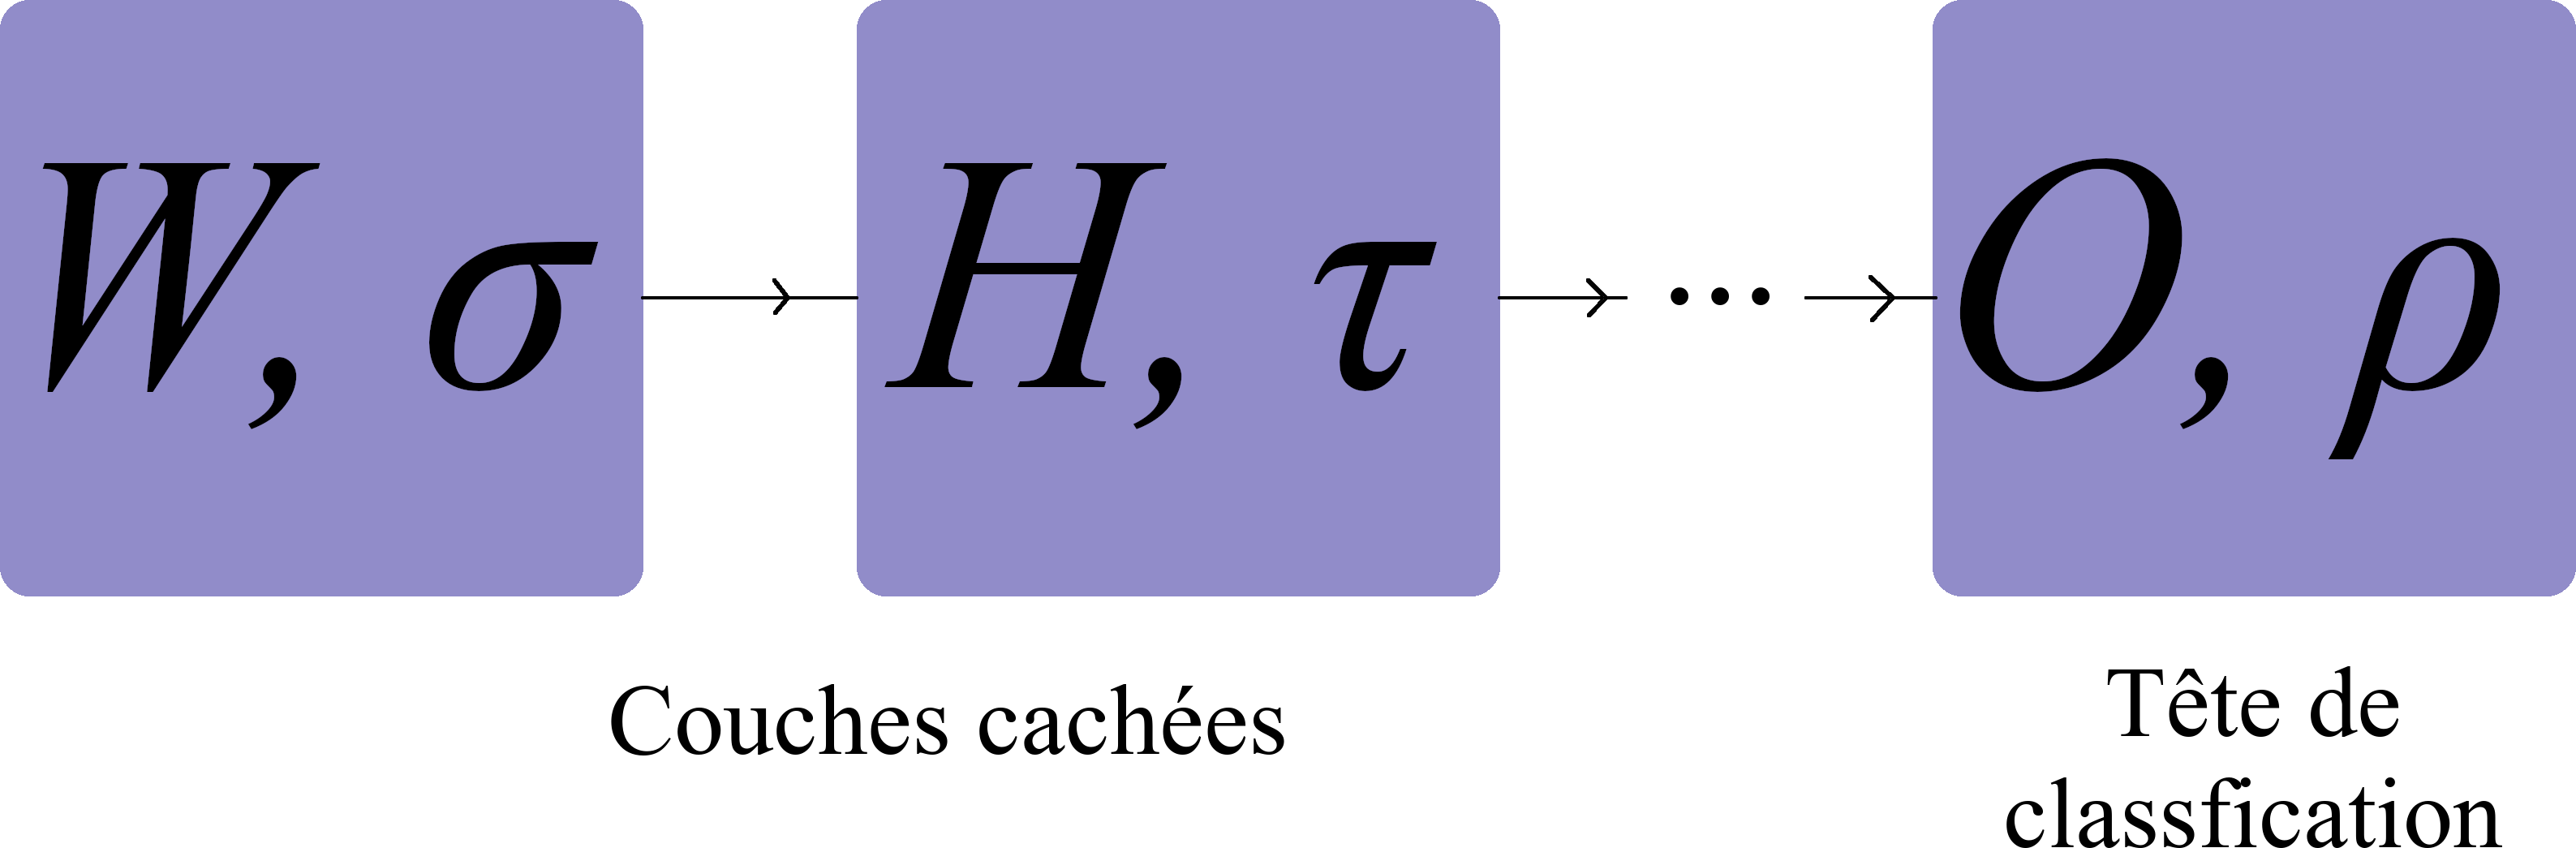
\includegraphics[width=\textwidth]{figures/ffnn.png}
    \end{subfigure}\hspace{0,5cm}
    \begin{subfigure}[b]{0.4\textwidth}
        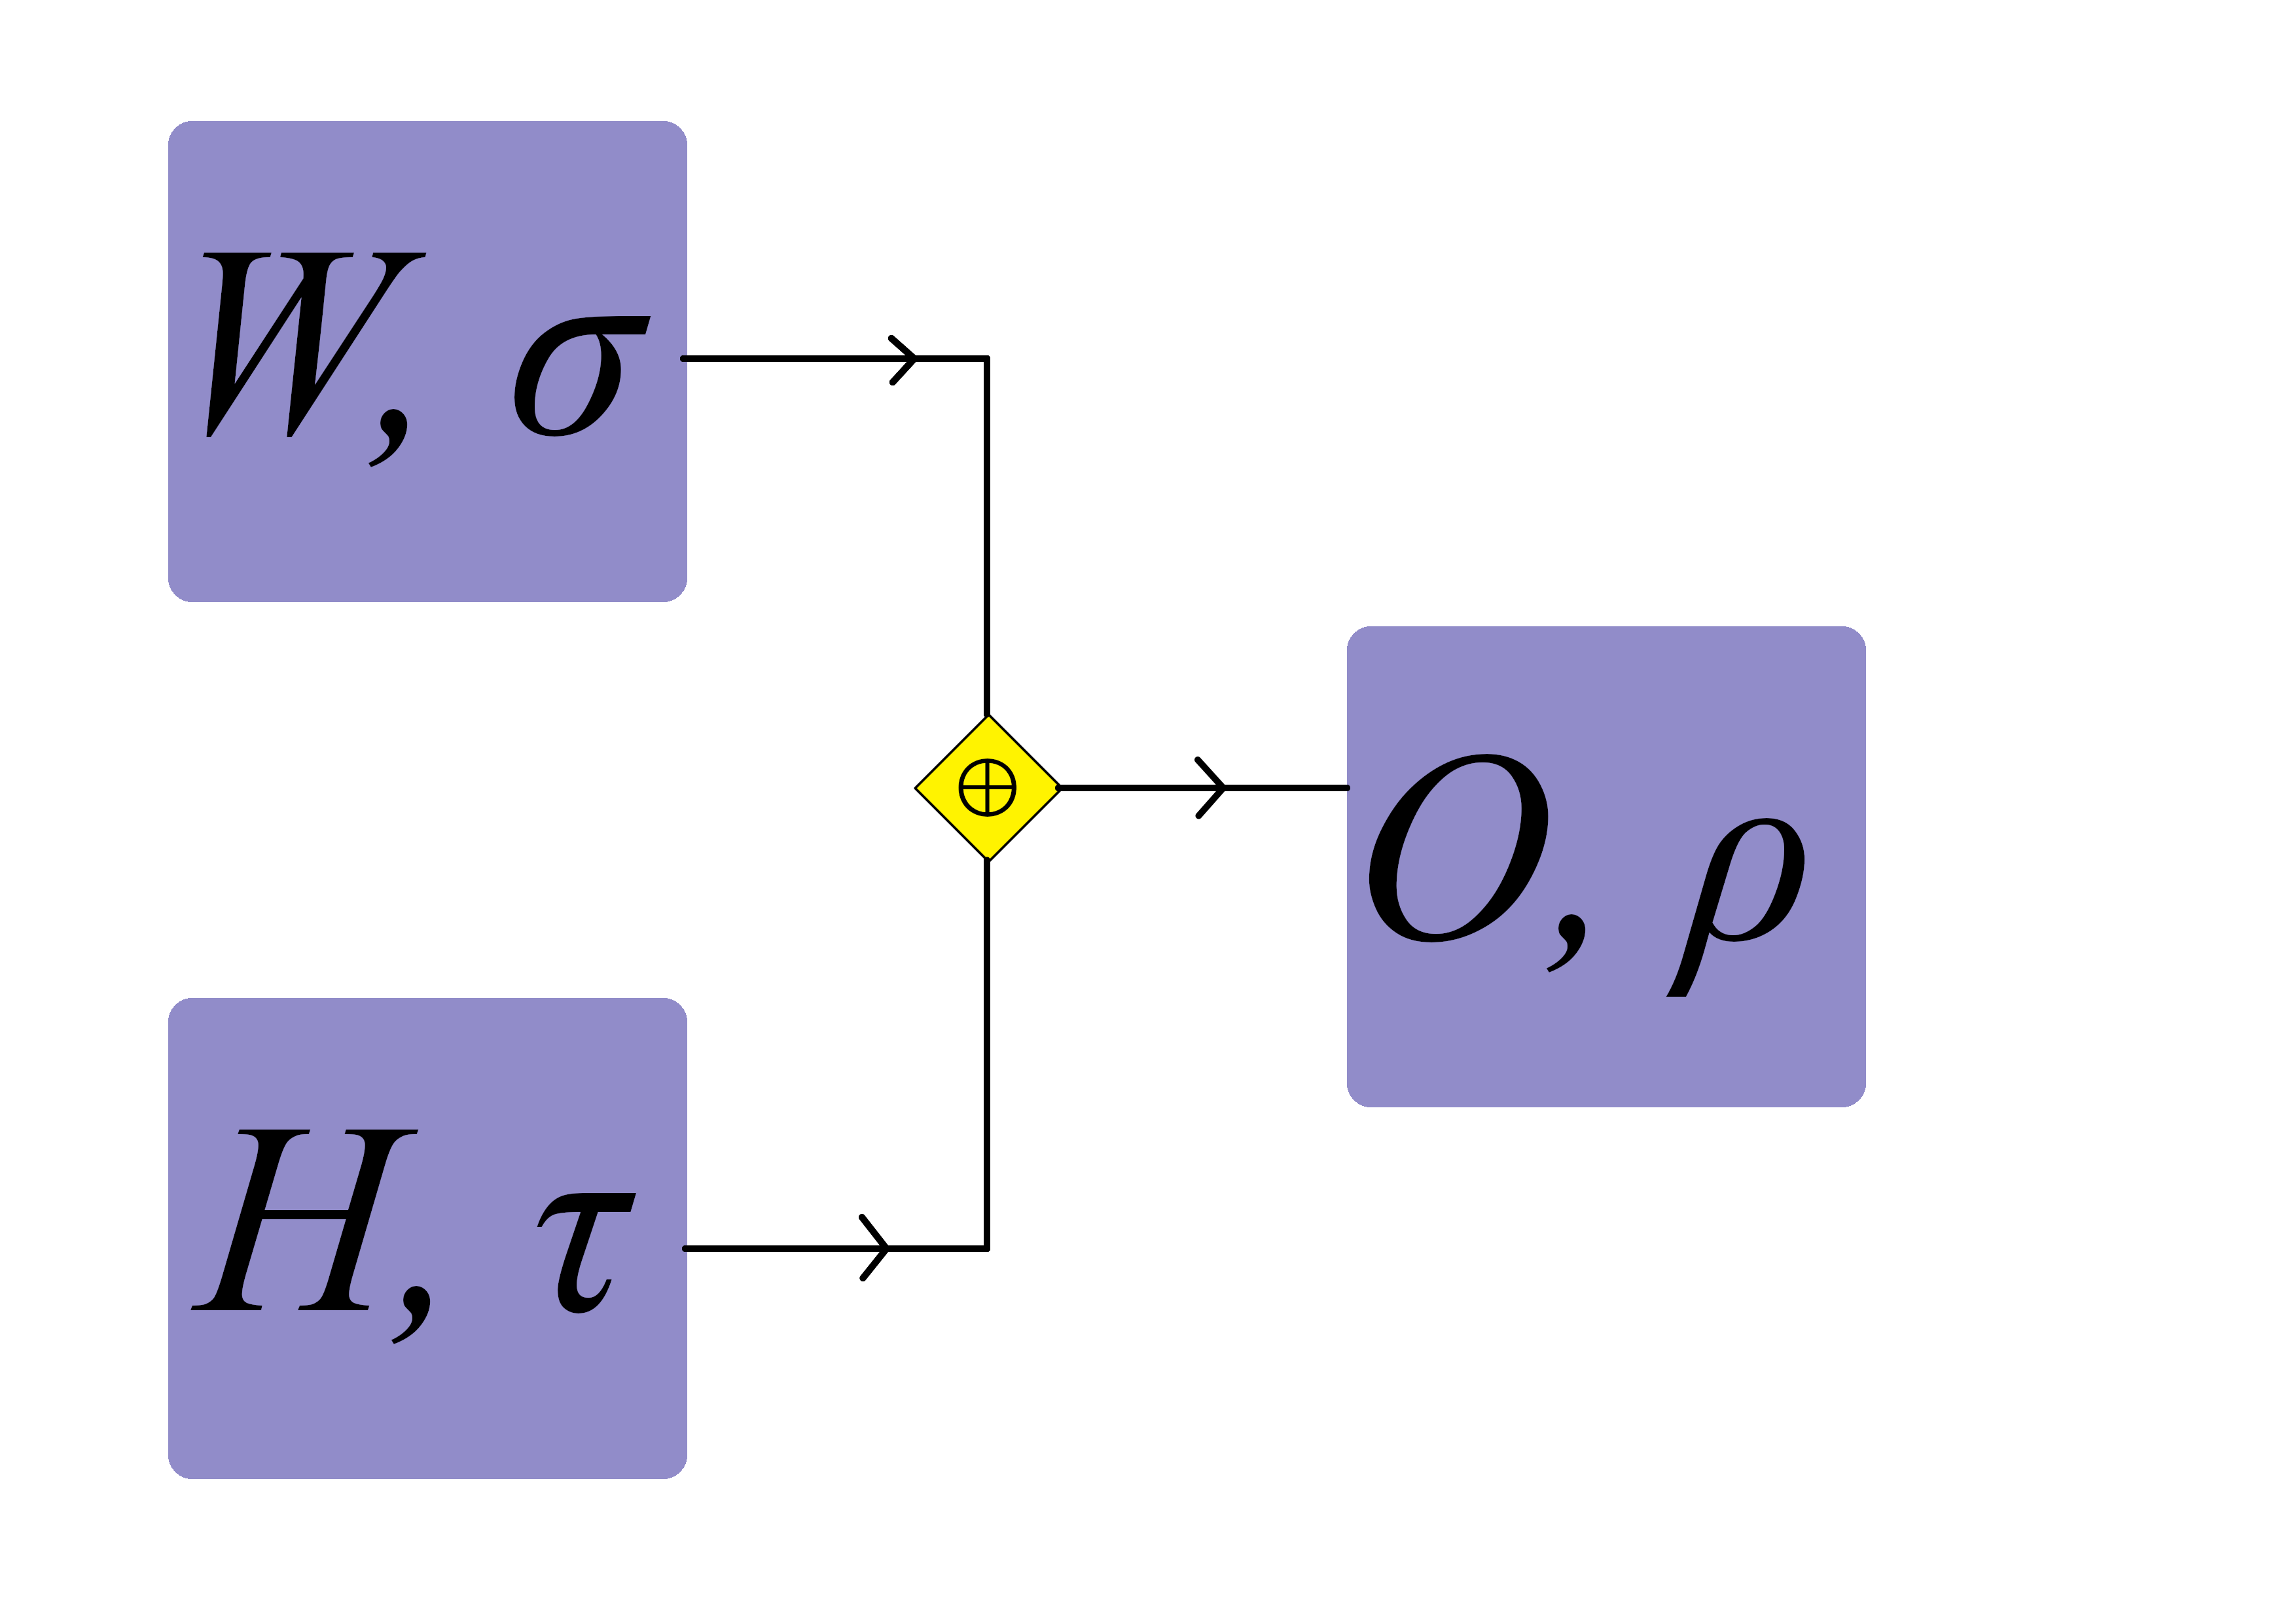
\includegraphics[width=\textwidth]{figures/arrangement_couches.png}
    \end{subfigure}
    \caption{Schéma de deux architectures possibles de réseaux de neurones. À gauche est représenté l'empilement le plus simple de couches neuronales, qu'on désigne par le terme de \og{} réseau de neurones à propagation avant \fg{}. À droite, une manière de combiner les informations de couches séparées -- ici par concaténation vectorielle -- a été schématisée.}
\end{figure}

% Parfait !

\subsubsection{Processus d'apprentissage}
% Exprimer le but de l'entraînement, qu'est que cela permet ? A chaque itération ?
L'entraînement d'un réseau de neurones s'effectue à travers des \textbf{ajustements des poids et des biais dans chaque couche}, dans le cadre d'une \textbf{minimisation d'une fonction de perte}\footnote{aussi appelée fonction de coût, ou d'erreur}. Cette fonction doit être choisie judicieusement selon le problème puisqu'elle exprime l'écart entre les sorties prédites et les sorties ciblées au passage de données d'entrée d'entraînement. Sa minimisation est réalisée par un algorithme de \textbf{descente du gradient}, avec le gradient de la fonction de perte selon tous les poids du réseau qui est calculé grâce à un procédé de \textbf{rétropropagation de l'erreur}, une adaptation pour les réseaux de neurones de celui de la discrimination rétropropagative pour des graphes d'exécution quelconques. Plusieurs implémentations de cet algorithme, qu'on nomme des \textbf{optimiseurs}\footnote{Adam \autocite{kingma2017adam} en est un assez connu et est celui qui était prévu d'être utilisé pour le codage de l'expérience.}, existent et la nature de l'optimiseur dans un modèle fait partie de ses paramètres d'entraînement.
% Petit graphique, exemple, pour s'imaginer le processus qui introduit bcp de nouveautés.

% Qu'est qu'un hyperparamètre ? - pas besoin de le définir
Des hyperparamètres pour l'entraînement sont également amenés à être définis en pratique, tels que le \textbf{taux d'apprentissage}, fixant la valeur maximale de variation qu'un poids ou biais peut subir au cours d'une rétropropagation, le nombre d'\textbf{époques} (\textit{epochs}), i.e. de balayages de l'ensemble des données du set d'entraînement pour l'exécution des descentes, et enfin la taille des \textbf{lots (\textit{batchs})}, i.e. des groupes de données d'entraînement à envoyer au modèle en une fois\footnote{Cette quantité est pensée pour prévenir les problèmes de saturation de la mémoire des ordinateurs, qui sont favorisés par les ordres de grandeur souvent importante des tailles des jeux de données d'entraînement.} \autocite[chap.~7, p.~17-23]{jurafsky}\autocite[21]{fourrier}.

\subsubsection{Concevoir correctement}
L'évaluation d'un modèle neuronal nécessite un jeu de données dont la nature dépend du problème à résoudre. En \Gls{tal}, du fait de la diversité des structures rencontrées dans une langue, les données doivent être capables de passer en revue un large éventail de cas pour vérifier que de bonnes généralisations aient été faites par la machine. Pour la même raison, quantifier la qualité des résultats prédits pour comparer plusieurs modèles nécessite d'établir une métrique avec parcimonie. \autocite[p. 43]{fourrier} Un exemple d'évaluation est synthétisé dans la sous-section \ref{descr_meloni}. \\
Le choix des paramètres d'un réseau de neurones pour améliorer sa capacité à pertinemment réaliser une certaine tâche ne se justifie \textit{a priori} que par l'expérience. \autocite[p.40]{fourrier} Il est néanmoins bon de noter que des recherches ont été menées pour automatiser le réglage de certaines configurations, comme par exemple celles de \cite{auto_sizing_layer_dim}, qui ont étudié des algorithmes pour trouver les dimensions minimales de couches cachées d'un \gls{modele_langue} neuronal aux performances fixées.

\subsection{Traitement des données}

Avant de donner à un réseau de neurones des données au format quelconque, que ce soit pour son entraînement ou pour réaliser des inférences dessus, il est nécessaire de les prétraiter. Le but est de les rendre correctes et compréhensibles pour un traitement numérique. Leur transformation se fait selon le type de tâche souhaitée. Néanmoins, dans sa généralité, les étapes de préparation des données en \Gls{tal} restent les mêmes.\\

\subsubsection{Normalisation}
Tout d'abord, il faut normaliser (nettoyer) la base de données qui peut être, par exemple, un corpus de textes, une liste de mots, provenant de la toile, ou d'un système de transcription audio-visuelle. Dans ces données se trouvent des chaînes de caractères sous un certain format, où de la ponctuation peut apparaître, de même que des lettres en capitale, des chiffres, des caractères spéciaux (comme le dièse que l'on retrouve souvent dans les \textit{tweets})... Mais une partie de ces éléments peut ne pas avoir d'intérêt à être traitée par les algorithmes ou peut même apporter du bruit aux données d'entraînement pour l'intelligence artificielle. Une première étape consiste à les supprimer ou bien à apporter des modifications à l'aide d'outils de traitement de texte\footnote{Par exemple, les Expressions Régulières (\textit{REGEX} pour \textit{Regular Expression}) est un outil puissant pour manipuler le contenu textuel. Un autre exemple est la librairie Python \url{https://www.nltk.org/} fournissant une variété de méthodes et d'outils pour traiter du texte.} \autocite[chap.~2]{jurafsky}.\\

\subsubsection{Tokenisation}
Après avoir nettoyé la base de données, il faut définir une segmentation des textes en éléments d'entrée pertinents pour faciliter le traitement par l'\Gls{ia} : les \glspl{token}. La tokenisation correspond à la segmentation de chaînes de caractères (comme notre texte) en tokens (mots, sous-mots, caractères, ponctuations). L'ensemble des tokens uniques d'un texte se nomme : vocabulaire.\\
\indent Prenons un exemple \og J'aime les bananes\fg, l'approche traditionnelle est de tokeniser notre texte suivant les blancs et les signes de ponctuation \footnote{Vous remarquerez déjà que ce processus ne s'applique pas aux langues, comme le Japonais ou le Chinois, manquant d'espace entre les caractères.} ce qui nous donne les tokens [\og J\fg, \og '\fg, \og aime\fg, \og les \fg, \og bananes\fg, \og .\fg] avec un vocabulaire de taille 6 (dans cette phrase tous les tokens sont uniques).\\
\indent Néanmoins, dans certains cas, cette approche peut être insuffisante, par exemple, lorsque les mots ne sont pas séparés ou lorsque la quantité de mots différents est importante. Ainsi, une technique récente vient compléter l'approche traditionnelle en segmentant un texte en sous-unités linguistiques, appelées sous-mots. Par exemple, le mot \og bananes\fg{} sera segmenté en deux tokens [\og banane\fg, \og s\fg]. Cette méthode peut s'approcher de deux façons, soit par l'application de \textit{règles} (adaptées à la langue) pour découper notre texte en sous mots (comme avec le mot \og bananes\fg{} dont on sait qu'en français le \og s\fg{} indique, pour un nom, le pluriel), soit par un algorithme purement statique segmentant de plus en plus un mot en sous-mots au fil que fréquence diminue dans le texte, dont l'un des plus connues pour ses performances et sa simplicité de mise en place est le \textit{Byte-Pair Encoding} (BPE) \autocite{bpe}\footnote{Il est bon de citer trois autres algorithmes qui sont tout aussi connues : \textit{unigram language modeling} \autocite{unigramkudo2018}, \textit{WordPiece}  \autocite{wordpiece}, \textit{SentencePiece} \autocite{sentencepiece} qui est une implémentation du BPE et de l'\textit{unigram language modeling}.}.

\subsubsection{Encodage}
Enfin, après avoir tokenisé un texte, il faut convertir ses tokens en vecteurs, car une machine, un réseau de neurones, ne comprend que des nombres et ne sait procéder qu'à des calculs. Il existe différentes façons de convertir un \gls{token} en un vecteur numérique, mais on retiendra deux méthodes : l'encodage \textit{one-hot} (ou 1 parmi $n$) et le plongement lexical (\textit{word embedding}).\\

L'encodage \textit{one-hot} consiste à créer un vecteur binaire de la taille du vocabulaire $|V|$, c'est-à-dire, que chaque dimension correspond à un mot (ou sous-mots)\footnote{Remarque : la dimension du vecteur dépend du degré de segmentation en sous-mots.} dans le vocabulaire. Dans ce vecteur binaire, la valeur est 1 pour la dimension correspondant au mot (ou sous-mot) dans le vocabulaire, et 0 pour toutes les autres dimensions. Ainsi, en supposant que la dimension du mot \og bananes\fg{} se trouve à la troisième dimension (c'est le troisième mot de notre vocabulaire $V$), sa représentation correspondra à un 1 à la troisième dimension du vecteur et à des 0 sur les autres dimensions, soit le vecteur :
\begin{align*}
    \begin{bmatrix}
    0 & 0 & 1 & 0 & \dots & 0
    \end{bmatrix}\\
    \begin{matrix}
    1 & 2 & 3 & 4 & \dots & |V|
    \end{matrix}
\end{align*}
\hfill \autocite[Chap 7]{jurafsky}\\

Comme vous pouvez le voir l'avantage de cet encodage est sa simplicité de mise en \oe{}uvre. Mais le problème survient quand le vocabulaire devient très grand, les vecteurs générés, par définition, deviennent à leurs tours très grands (le nombre de dimension pour décrire les données augmente) et très dispersés (beaucoup de 0 et peu de 1), ce qui entraîne une augmentation de la complexité et des temps de calcul. De plus, cet encodage ne prend pas en compte les relations sémantiques entre les mots, la similarité entre deux mots ne peut être mesuré,  car ils sont encodés de façon indépendante les uns des autres, ce qui peut être particulièrement problématique pour les nombreuses tâches de \Gls{tal} tel que la compréhension ou traduction d'une langue.\\

Le plongement lexical, en revanche, permet de représenter les mots en encapsulant leur \textit{sens sémantique} par des vecteurs denses de plus faibles dimensions, c'est à dire des vecteurs de nombres réels de petites tailles. Pour obtenir le plongement des tokens, c'est-à-dire, transformer des tokens en vecteurs, une matrice de plongement est utilisée\footnote{Techniquement, la conversion s'effectue d'abord par un plongement en \textit{one-hot} qui est ensuite converti en plongement lexical via la multiplication matricielle en théorie, mais via un tableau de correspondance (entre les mots et leur plongement lexical) en pratique}, obtenus par l'entraînement d'un modèle\footnote{Généralement, l'entraînement s'effectue de façon non supervisée à partir d'un grand corpus de texte, pour permettre au modèle de se représenter les relations sémantiques et syntaxiques qui peuvent exister entre les mots. Nous pouvons citer, comme exemples de modèles, Word2Vec et GloVe qui sont souvent utilisés pour créer des matrices de plongement lexical. Une méthode plus moderne consiste à apprendre les plongements directement à l'intérieur du modèle, comme le modèle Bert. Pour approfondir le sujet, nous vous invitons à regarder \autocite[chap.~6, 7, 11]{jurafsky}.}. Cette matrice contient, à chaque ligne, le plongement d'un \gls{token} du vocabulaire, et à chaque colonne correspond une dimension du vecteur de plongement. Par ailleurs, les dimensions de ces vecteurs n'ont pas une représentation claire \autocite[chap.~6]{jurafsky}. Comme cette matrice représente un espace vectoriel, ainsi, les propriétés vectorielles peuvent s'appliquer pour nos tokens vectorisés. Par exemple, étudier la similarité entre deux mots revient à calculer la distance entre les deux vecteurs correspondants, ou encore comme la figure \ref{fig:wordvec} le montre, les vecteurs peuvent s'additionner/se soustraire permettant d'obtenir un nouveau vecteur qui garde une cohérence sémantique face à ces opérations. \autocite{rumel} \autocite{lund}

\begin{figure}[!h]
    \centering
    \begin{subfigure}[b]{0.6\textwidth}
        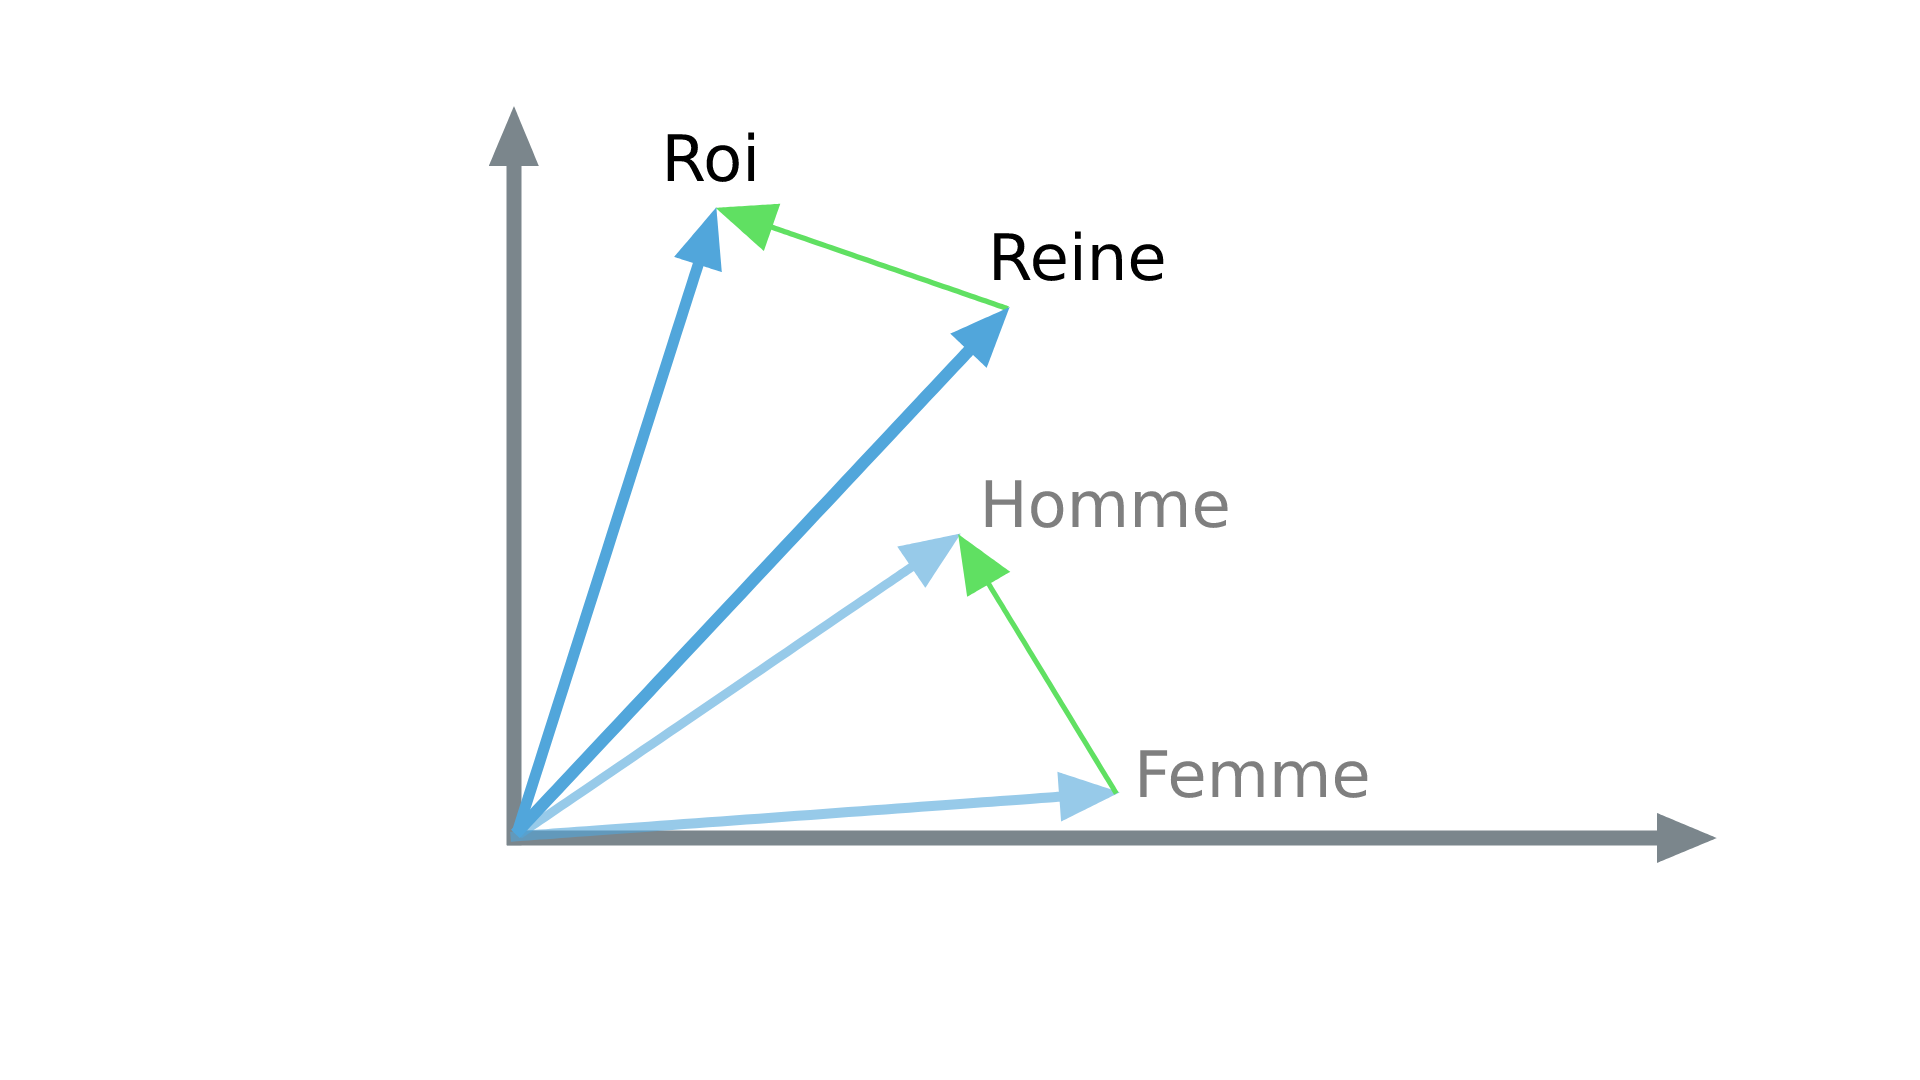
\includegraphics[width=\textwidth]{figures/word_vec.png}
    \end{subfigure}
    \caption{Analogie connu montrant les relations sémantiques et algébriques entre les mots dans un espace de plongement lexical. La soustraction du vecteur $\overrightarrow{Femme}$ avec l'addition du vecteur $\overrightarrow{Homme}$ permet d'obtenir le vecteur vert entre ces deux vecteurs. Et en appliquant ce nouveau vecteur au vecteur $\overrightarrow{Reine}$, on obtient le vecteur $\overrightarrow{Roi}$.}
    \label{fig:wordvec}
\end{figure}

\newpage
\subsection{Architectures neuronales utiles au TAL}

En \Gls{tal}, le besoin d'identifier des informations \textbf{contextuelles} s'est fait ressentir. Pour par exemple relever des diphtongues, dans une tâche de modélisation du changement phonétique, un réseau de neurones devra traiter des \textbf{séquences} de \glspl{token} représentant des décompositions de mots en chacun de leurs sons, et ensuite apprendre à établir des liens entre les \glspl{token}.\\
Une bonne intuition est que des représentations calculées en profondeur dans un réseau de neurones pour certains éléments de la séquence seront utiles pour le calcul de prédictions sur d'autres éléments de cette même séquence. 

Dans cette section, des types d'architectures vont être présentés pour leur capacité à construire de manière puissante des contextes dans des séquences d'information.
\subsubsection{Réseaux de neurones récurrents} \label{rnn_def}

Les Réseaux de Neurones Récurrents (\textit{Recurrent Neural Networks} (\Gls{rnn})) permettent de prendre en compte un contexte. Étant donné une séquence de $n$ entrées $(x_i)_{1\leq i \leq n}$, le \Gls{rnn} le plus élémentaire est un enchaînement d'une couche cachée avec une autre couche.\autocite{origine_srnn} La sortie est alors inférée comme dans l'équation \ref{eq:def_rnn} Les vecteurs des biais seront dorénavant gardés implicites dans les expressions afin de les simplifier.
\begin{equation} \label{eq:def_rnn}
    y_i = \sigma(Vh_i)
\end{equation}
La valeur ajoutée du \Gls{rnn} réside dans le calcul de cette couche cachée, qui en plus d'être une fonction de l'entrée $x_i$ de la séquence est également une fonction de la couche cachée qui a été calculée en ayant passé en revue les éléments précédents de la séquence. Une somme pondérée des deux vecteurs est alors effectuée dans la définition de $h_i$, ce pourquoi deux matrices de poids interviennent :
\begin{equation}
    h_i = \sigma'(Hh_{i-1} + Wx_i)
\end{equation}

La propagation du flux d'informations amenant à la sortie d'un modèle RNN pour un certain élément d'une séquence d'entrée peut être illustrée avec le figuré \ref{fig:rnn}. Avec la simplification faite dans le schéma, on remarque aisément qu'on peut construire des empilements d'unités RNN, de la même manière qu'on approfondit l'apprentissage en empilant des couches plus simples.\autocite[chap.~9, p. 1-4]{jurafsky}

\begin{figure}[!h]
    \centering
    \begin{subfigure}[b]{0.3\textwidth}
        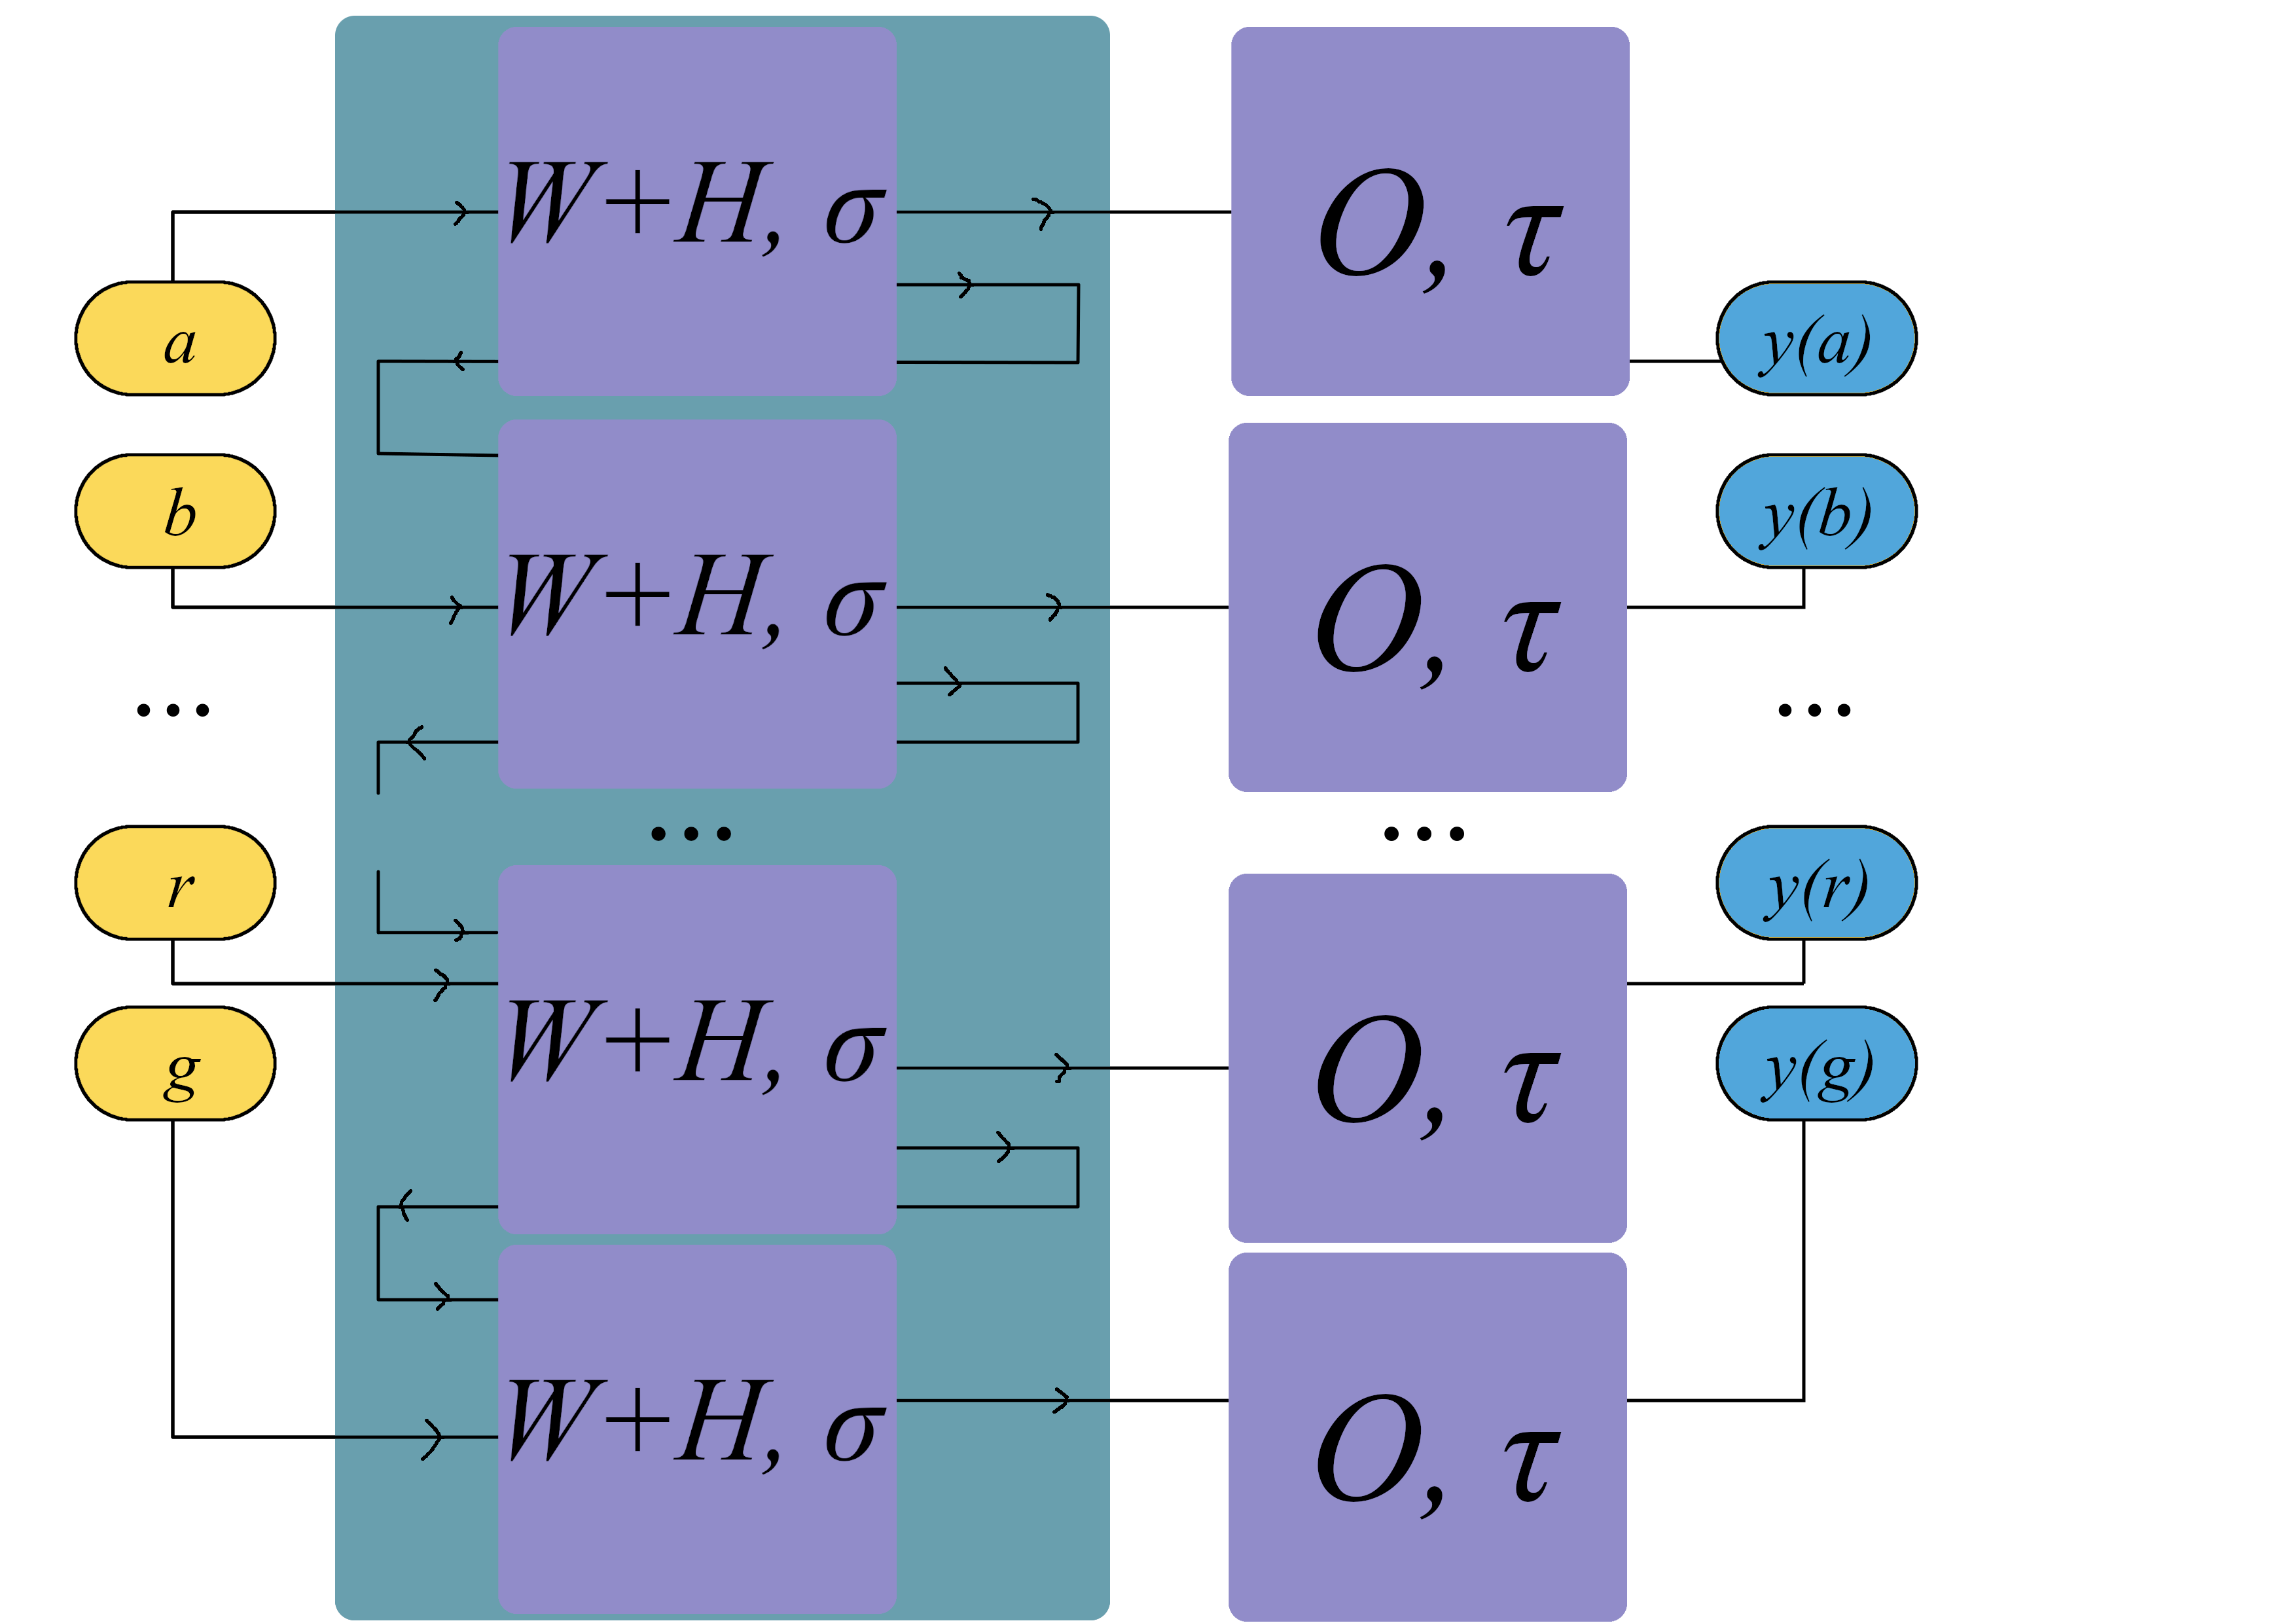
\includegraphics[width=\textwidth]{figures/rnn.png}
    \end{subfigure}
    \begin{subfigure}[b]{0.4\textwidth}
        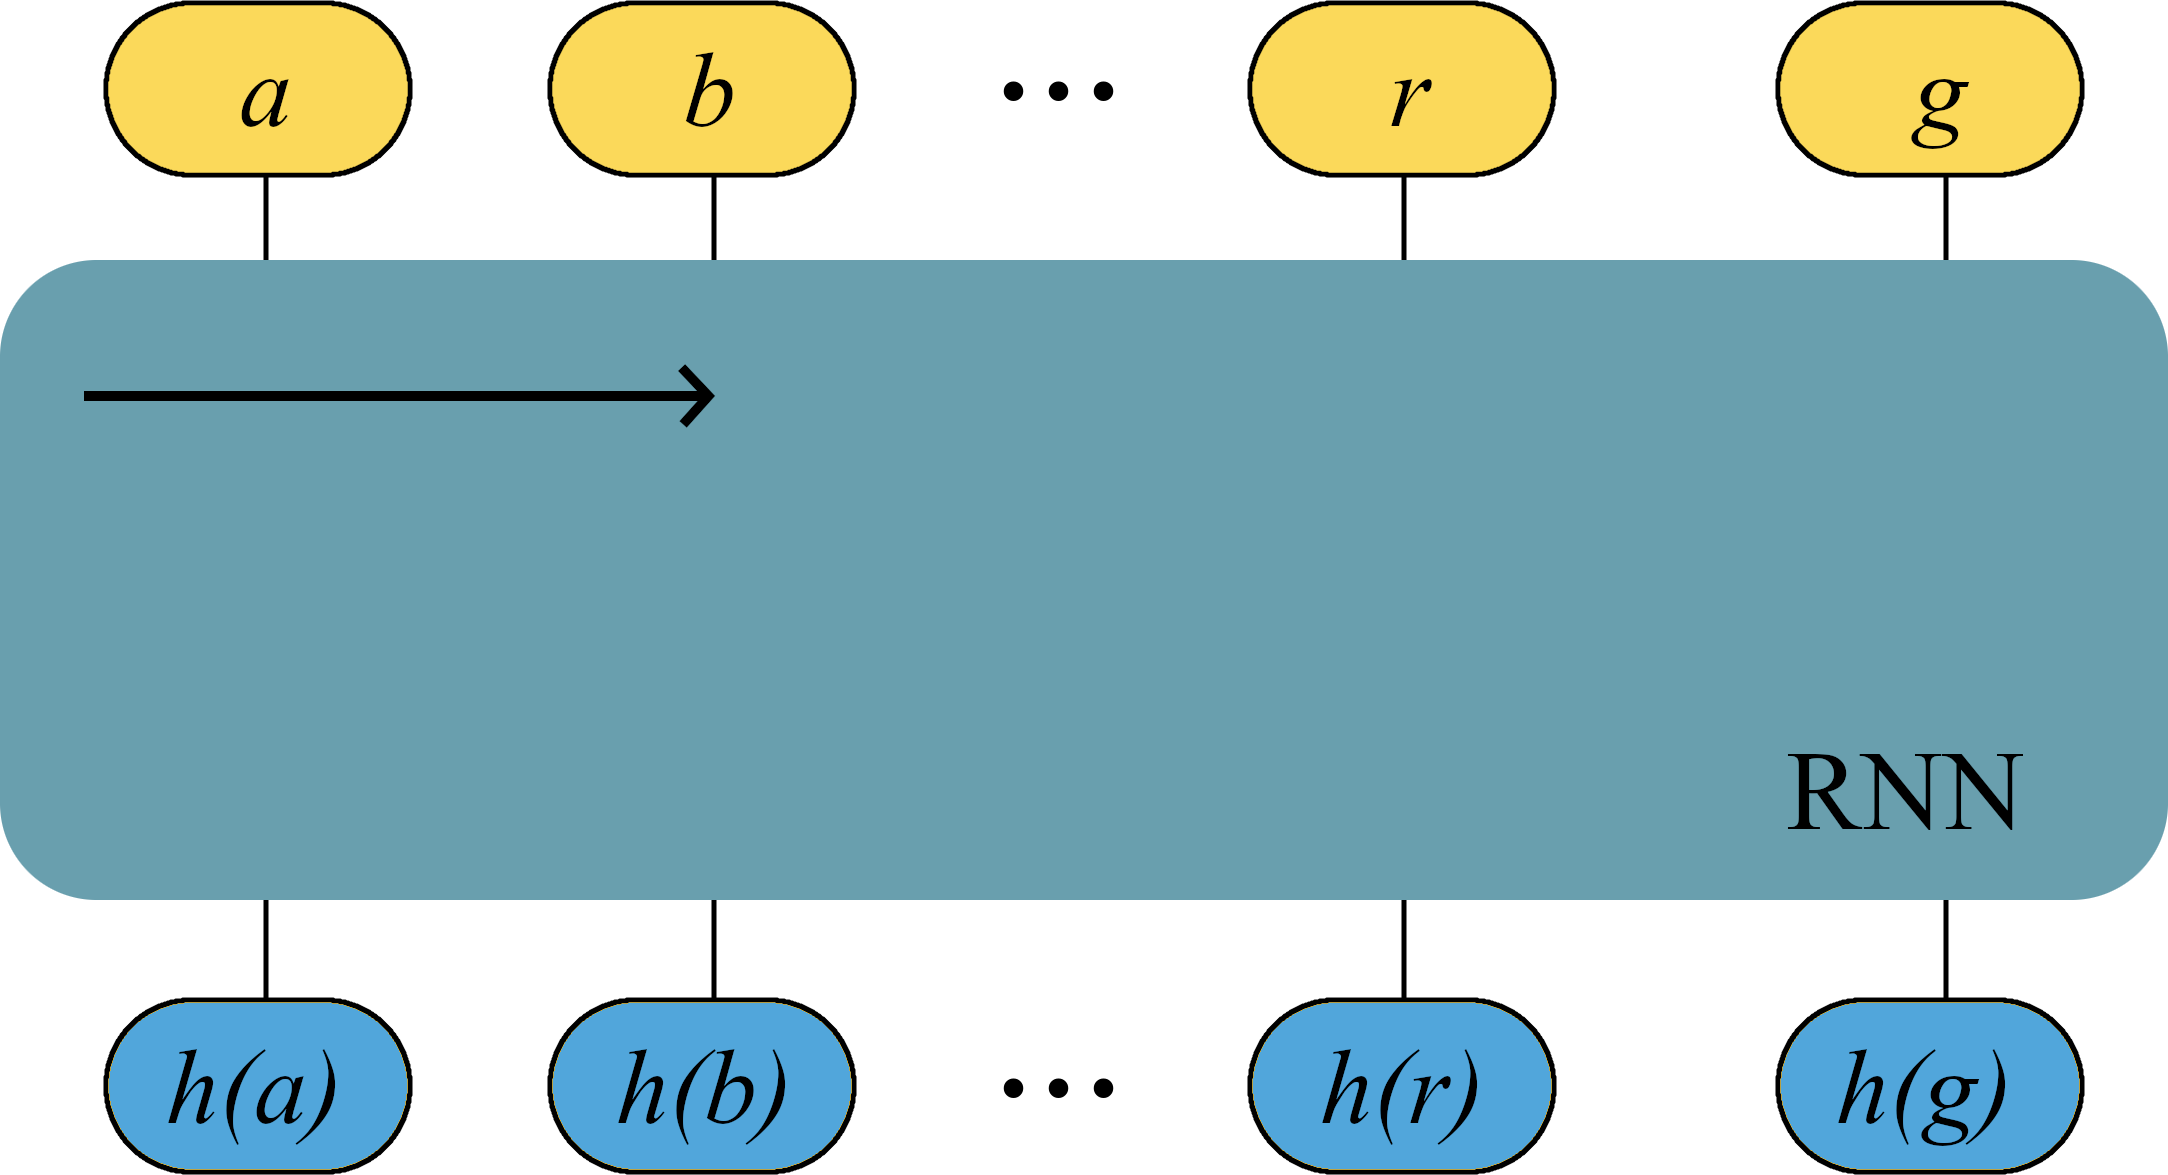
\includegraphics[width=\textwidth]{figures/rnn simp.png}
    \end{subfigure}
    \caption{Schématisation d'un réseau de neurones récurrent. À droite, il est montré qu'il est possible de directement exploiter les vecteurs cachés, sortis par la couche RNN. Ces derniers sont d'une dimension arbitraire, à définir avec l'unité de RNN.}
    \label{fig:rnn}
\end{figure}

Dans ces schémas, la séquence d'entrées n'a été parcourue que de gauche à droite, mais il existe des problèmes, comme celui mentionné en introduction de cette section, où le contexte à gauche comme à droite d'un élément de la séquence doit être pris en compte. Une configuration architecturale des RNNs peut justement permettre de construire des contextes de manière \textit{bidirectionnelle} \autocite{bi_rnn}. Dans celle-ci, la couche cachée pour l'entrée $x_i$ est produite à partir de la concaténation des couches cachées ayant balayée respectivement les entrées $(x_1, x_2, ..., x_{i-1}, x_{i})$ et dans l'autre sens les entrées $(x_n, x_{n-1}, .., x_{i+1}, x_i)$. \autocite[chap.~9, p. 11-13]{jurafsky}

\begin{figure}[!h]
    \centering
    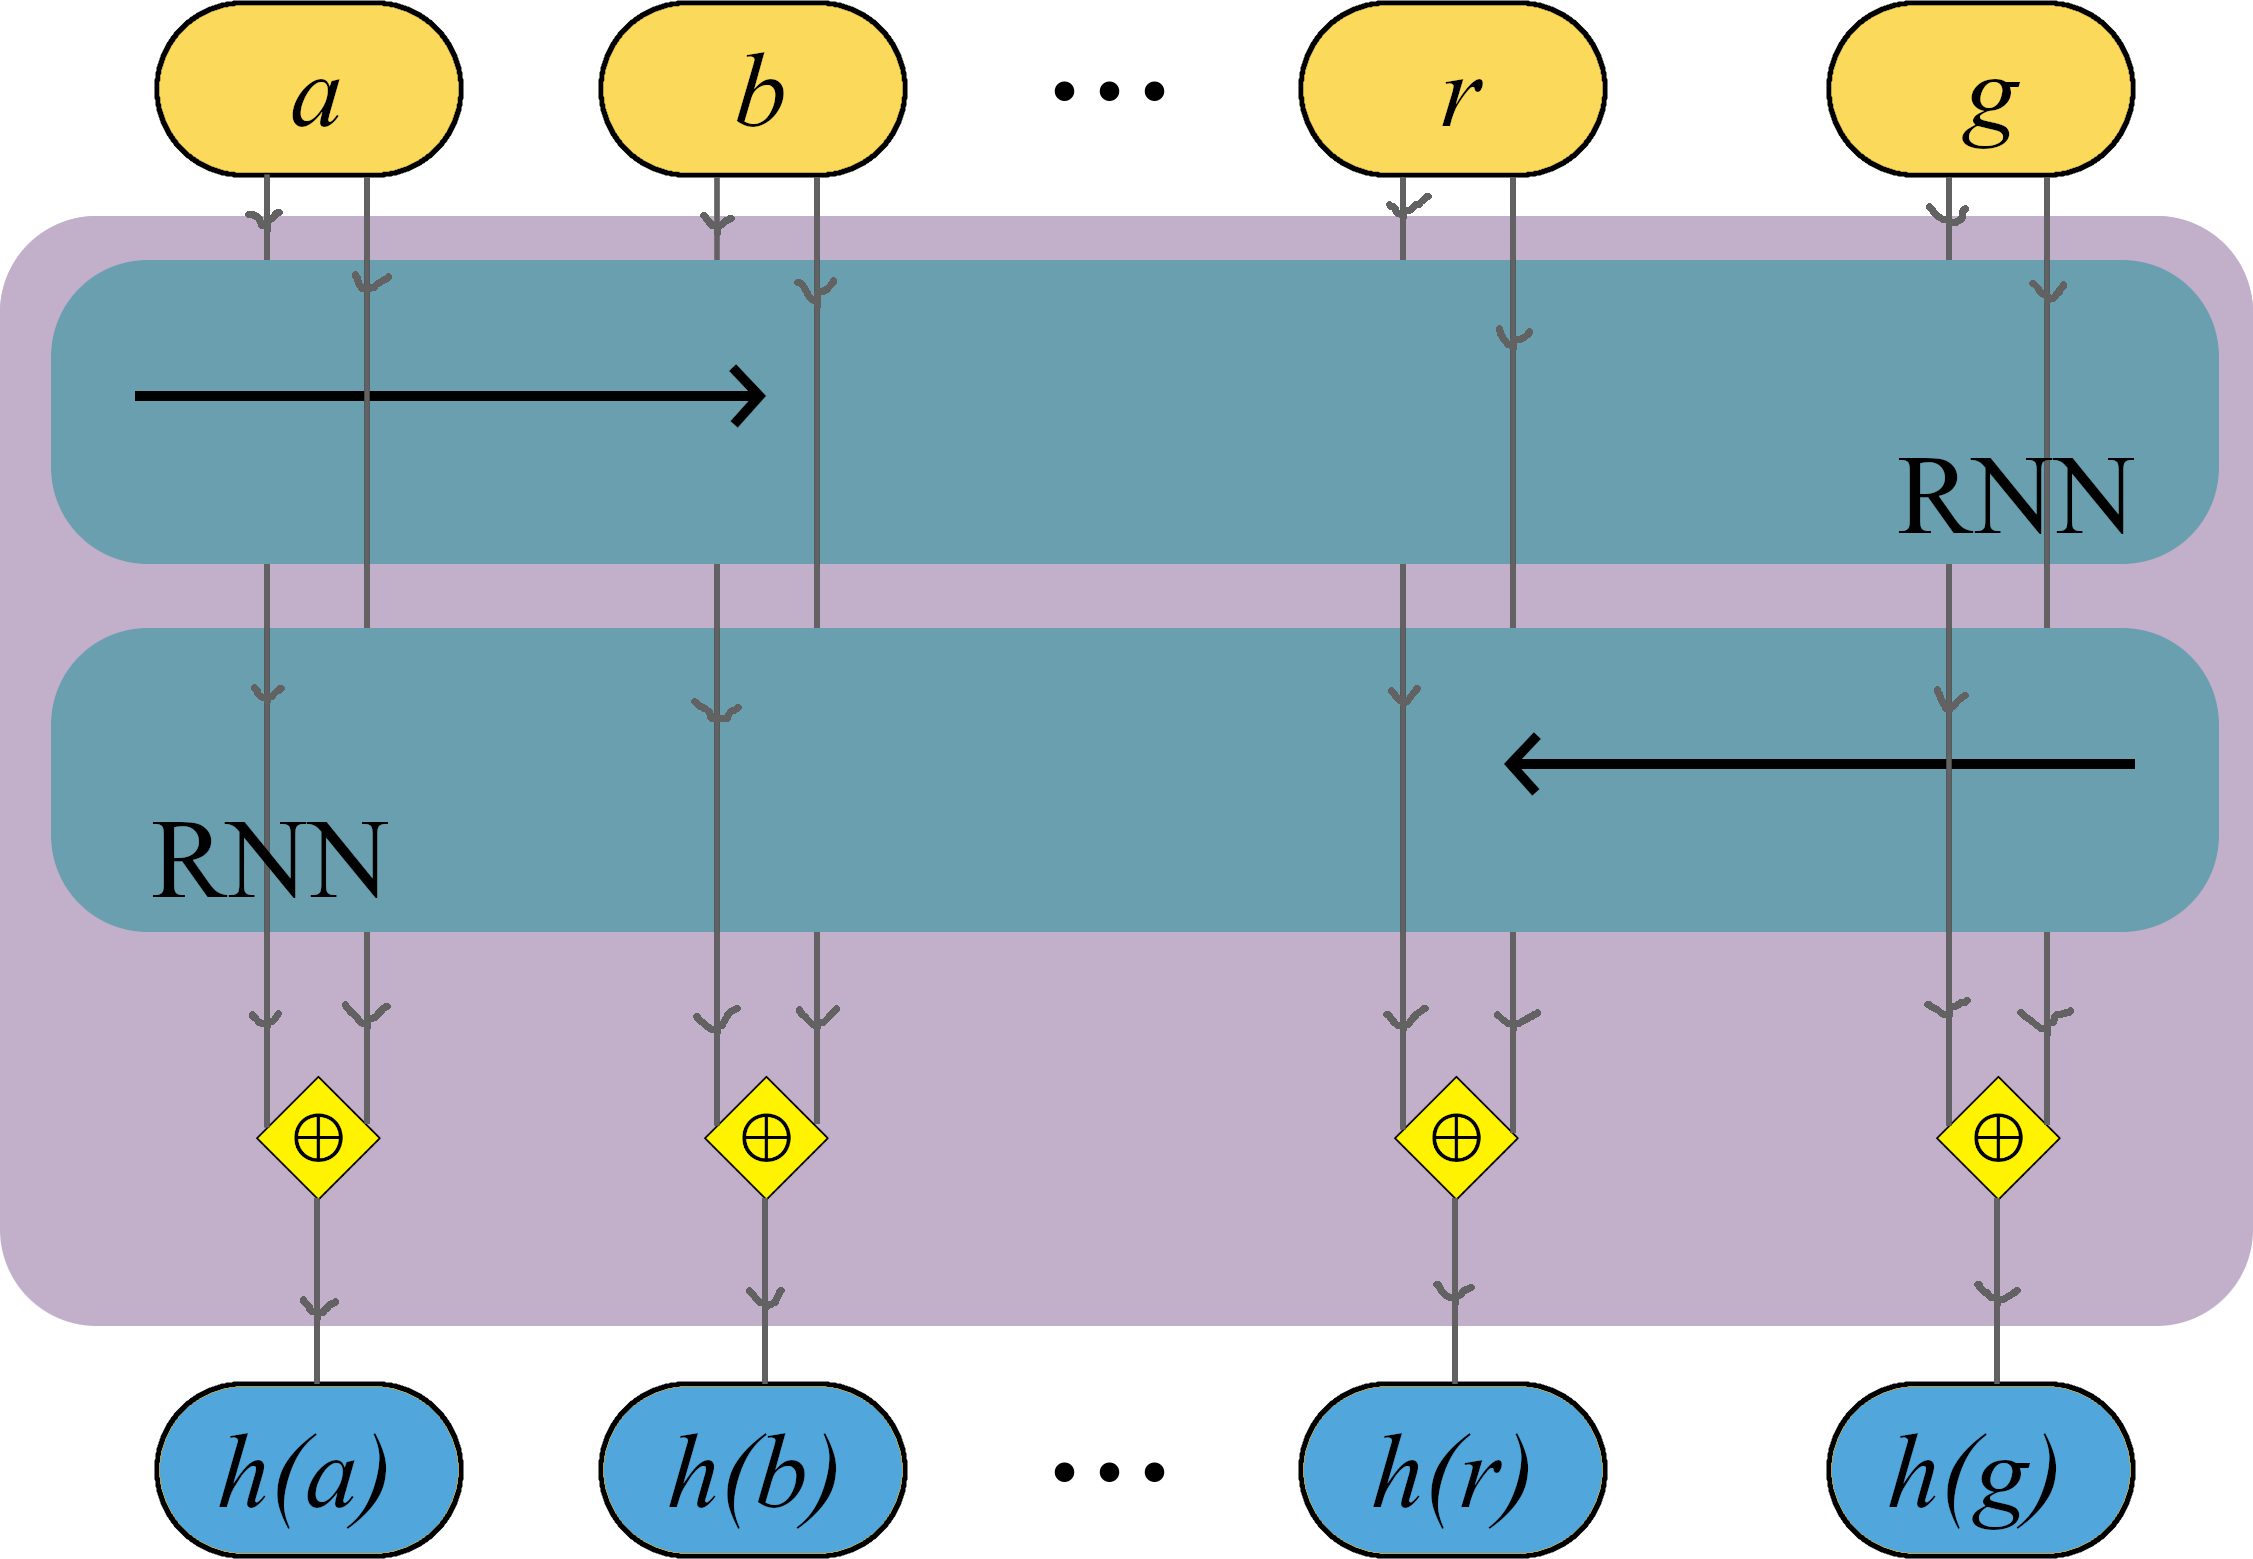
\includegraphics[width=0.3\textwidth]{figures/rrn_bidi.png}
    \caption{Schéma de la structure interne d'un RNN bidirectionnel.}
    \label{fig:rnn_bidi}
\end{figure}

Avec des séquences de tokens dans les données, les \Glspl{rnn} sont alors entraînables. En revanche, il a été observé que la rétropropagation du gradient ne se déroule pas correctement pour des séquences de taille trop importante, ce qui empêche ce type de réseau d'exploiter efficacement une information contextuelle se situant au-delà d'un certain voisinage autour du \gls{token} à traiter \autocite[p. 25-26]{fourrier}.

\subsubsection{Architecture \textit{Long Short-Term Memory}} \label{lstm_def}

Les \textit{Long Short-Term Memories}(\Glspl{lstm}) sont des modèles neuronaux dont l'architecture est une variante à celle des \Glspl{rnn} conçue expressément pour repousser les limitations de ces derniers. Le réseau de neurones est alors entraîné à focaliser son \textbf{attention} sur les bons éléments de contexte.

Une unité \Gls{lstm} est de ce fait plus complexe qu'une unité \Gls{rnn}, mais elle bénéficie de la même modularité. Ainsi, on peut empiler des \Glspl{lstm} et construire des \Glspl{lstm} bidirectionnels de la même manière que décrite plus tôt avec les \Glspl{rnn}.\\

La complexification architecturale peut dans un premier temps se remarquer d'un point de vue externe en notant que, là où une unité RNN n'est composée que d'une couche cachée qui est une fonction de l'entrée et d'une ou plusieurs couches cachées périphériques, l'unité LSTM est composée en plus d'une \textbf{couche de contexte} qu'elle renvoie et qui est utilisée pour le calcul des couches cachées et de contexte des autres entrées dans la séquence.

D'un point de vue interne, ces deux couches interagissent à travers des \textbf{portes} qui sont entraînées pour rejeter de l'information tout en promouvant d'autre. \autocite[cf.][chap. 9, p. 14-16]{jurafsky}

\subsubsection{Transformeurs} \label{transformers}

Un type de réseau de neurones a été introduit il y a moins d'une décennie en ayant surpassé les difficultés de parallélisation causées par les connexions récurrentes des modèles introduits précédemment : le \textit{Transformer} (Transformeur en français) \autocite{transformer}. Ce modèle de type encodeur-décodeur se base sur un mécanisme d'\textbf{attention multi-têtes}\footnote{Par simplification, nos efforts se concentrerons sur l'attention multi-têtes, en ignorant la décomposition en blocs de \textit{transformer}, contenant chacun une unité d'attention multi-têtes (masqué ou non) ainsi qu'une tête de classification, accompagné de connexions résiduelles et de couches de normalisation \cite[pour plus de détails, voir][{}]{transformer}.}.\\

L'attention multi-têtes permet d'étudier tous les vecteurs d'entrées, comme des mots, en même temps (de façon parallèle). Chaque tête qui la compose se focalise sur un aspect des \textit{interactions} entre les différents éléments de la séquence. Par exemple, dans la phrase \og Toto aime les bananes vertes\fg{}, un tête fera attention à \textit{qui} aime (\og Toto\fg{}), une autre à l'objet aimé \og les bananes\fg{}, et encore une à l'adjectif utilisé pour l'objet (\og vertes\fg{}).\\ 

Une tête contient un module d'auto-attention (\textit{self-attention}) qui est utilisé pour identifier les interactions de chaque \gls{token} $x_i$ avec tous les autres de la séquence $X=(x_1, x_2, \dots, x_n)$. Ceci est permis grâce au calcul d'un trio de vecteur pour chaque $x_i$ : un vecteur de requête (\textit{query}) $q_i$, un de clé (\textit{key}) $k_i$ et un de valeur (\textit{value}) $v_i$. Le vecteur requête $i$ correspond à celui sur lequel l'attention est portée et sera comparé à tous les vecteurs clés de la séquence ($j\ne i$). Le vecteur valeur sera ensuite multiplié par le poids d'attention calculé avec les autres vecteurs (requêtes et clés). Pour créer ces vecteurs, les vecteurs $x_i$ sont multipliés avec les matrices de poids ($W^Q$, $W^K$, $W^V$) qui sont obtenus à l'entraînement du modèle :
\begin{equation}
    q_i = W^Q x_i \quad ; \quad k_i = W^K x_i \quad ; \quad v_i = W^V x_i
\end{equation}
On pose l'ensemble des vecteurs $q_i$, $k_i$, $v_i$ sous forme de matrice, respectivement $Q$, $K$, $V$.\\

Ensuite, le calcul d'auto-attention pour une tête s'effectue par la multiplication du score d'attention $(QK^T)$, normalisé par la racine carré de la dimension $d_k$ de la matrice $Q$ et $K$, et par la fonction \textit{softmax}, avec la matrice des valeurs $V$ :
\begin{equation}
    Attention(Q, K, V) \quad  = \quad  softmax(\frac{QK^T}{\sqrt{d_k}})V
\end{equation}

Enfin, l'ensemble des matrices d'auto-attention correspondant à chaque tête est concaténé en une unique matrice qui est multipliée par une matrice de poids $W^O$ (également obtenus à l'entraînement) pour former la matrice résultante de l'attention multi-têtes :
\begin{equation}
    MultiHeadAttention(X) \quad = \quad Concat(head_1, head_2, ...)W^O
\end{equation}
\hfill où $head_i = Attention(Q_i, K_i, V_i)$\\
\vspace{2pt}
\hfill avec $Q_i = XW^Q_i$ ; $K_i = XW^K_i$ ; $V_i = XW^V_i$\\
\vspace{2pt}
\hfill et $i$ allant de $1$ au nombre de têtes définis.\\

Cependant, au tout début, il a été évoqué que le modèle étudiait l'ensemble des tokens $x_i$ en même simultanément. Ainsi, le modèle ne tient pas compte de l'ordre des tokens, une information pourtant capitale. Par conséquent, pour injecter l'information de la position de nos tokens dans les vecteurs d'entrées, le papier \cite{transformer} propose une solution en additionnant, à nos tokens plongés (vectorisés), des vecteurs positions créés à base de fonction sinus et cosinus \footnote{Nous invitons le lecteur à regarder le papier de \autocite{transformer} pour se convaincre de la pertinence de ce choix d'encodage de position. Simplement, retenez que cela permet au modèle de s'entraîner avec la position relative des tokens, plutôt que la position absolue.}. Cette méthode permet, ainsi, à notre modèle de travailler avec tous les tokens $x_i$, de notre séquence $X$, en même temps, tout en ayant l'information de leur position (dans la séquence) dans leur vecteur.\\

Dans certaines situations, notamment dans la tâche de modélisation du langage en \Gls{tal}, où le but est de prédire le prochain mot d'une phrase, l'entraînement avec ce type de Transformeur est assez inapproprié, car le mot suivant est déjà connu. Le modèle apprendra juste, à son entraînement, de renvoyer en sortie les tokens d'entrées. Pour résoudre ce problème, les chercheurs\footnote{Ils ont proposé cette variante car leur modèle de \textit{base} répondait aux problématiques des réseaux récurrents pour la traduction automatique.} proposent d'appliquer un masque qui remplacent par des $-\infty$ (qui seront transformés en 0 par la fonction \textit{softmax}) les valeurs de la partie triangulaire supérieure de la matrice $QK^T$ (le score d'attention). Cette variante se nomme l'auto-attention masquée. De ce fait, le champ de visibilité de notre modèle sera réduit au mot qu'il est en train de voir et à ceux qu'il a déjà vus, et pourra prédire de façon plus pertinente (sans triche) les prochains mots de la phrase.

\chapter{Les contributions de l'IA dans la linguistique historique}

Après avoir énoncé quelques principes de la linguistique historique et de l'intelligence artificielle dans le traitement automatique des langues, nous allons aborder des applications de l'intelligence artificielle à deux problématiques de la linguistique historique, la restauration de documents anciens et le déchiffrement de langues anciennes.

\section{Restauration de documents anciens}
% Ithaca
\indent La restauration d'inscriptions endommagées nécessite que les épigraphistes s'appuient sur de vastes bases de données pour trouver des parallèles textuels et contextuels. Ces référentiels sont principalement constitués du répertoire mnémotechnique des parallèles d'un chercheur et, plus récemment, de corpus numériques permettant d'effectuer des recherches par \og correspondance de chaînes de caractères\fg. Cependant, des différences dans la requête de recherche peuvent exclure ou obscurcir des résultats pertinents, et il est difficile -- voire impossible -- d'estimer la véritable distribution de probabilité des restaurations possibles. L'attribution d'une inscription pose aussi problème : si elle a été déplacée ou si des éléments de datation internes utiles manquent, les historiens doivent trouver d'autres critères pour attribuer le lieu et la date de l'écriture (formes de lettres, dialectes, etc). Et cela implique inévitablement, un niveau élevé de généralisation, les intervalles d'attribution chronologique pouvant être très longs.\\

Ainsi, l'utilisation d'un modèle de langue nommé Ithaca \autocite{deepmind2022} permet de surmonter les méthodes épigraphiques actuelles en utilisant l'apprentissage automatique sur de grandes quantités de données (quand celles-ci sont disponibles). L'augmentation récente de la puissance de calcul a permis à ces modèles de relever des défis de plus en plus sophistiqués dans de nombreux domaines, y compris l'étude des langues anciennes.
Ithaca est un réseau de neurones de type Transformeur, entraîné à effectuer simultanément les tâches de restauration textuelle, d'attribution géographique et d'attribution chronologique. Il a été formé sur des inscriptions écrites en grec ancien et dans le monde méditerranéen entre le VIIe et le XXe siècle. Ce choix s'explique par deux raisons principales. La variabilité du contenu et le contexte des documents épigraphiques grecs en fait un excellent défi pour le traitement des langues, de plus, la disponibilité de corpus numérisés pour le grec ancien est une ressource essentielle pour l'entraînement des modèles d'apprentissage automatique.\\

Pour commencer, le texte d'entrée est représenté sous forme conjointement de caractères et de mots, en remplaçant les mots endommagés, manquants ou inconnus (\textit{unknown}) par un symbole spécial \og [unk]\fg.\\
Ithaca utilise le mécanisme d'attention pour évaluer l'influence des différentes parties de l'entrée \cite{deepmind2022} (telles que les caractères, les mots) sur le processus de prise de décision du modèle. 
Le modèle est constitué de blocs de transformeur empilés : chaque bloc produit une séquence de représentations traitées dont la longueur est égale au nombre de caractères d'entrée, et la sortie de chaque bloc devient l'entrée du suivant. La sortie finale de l'ensemble des blocs est transmise à trois têtes\footnote{Il faut tenir compte du fait que ces têtes sont différentes de celles contenus dans les blocs de transformeur, les multi-têtes d'attention.} de tâches différentes qui traitent respectivement la restauration, l'attribution géographique et l'attribution chronologique. Chaque tête est constituée d'un réseau neuronal \textit{feedforward}, spécifiquement entraîné pour chaque tâche.\\

Ithaca est conçu pour assister et étendre le travail de l'historien. Seul, il a atteint une précision de 62\% lors de la restauration de textes endommagés, mais l'utilisation d'Ithaca par des historiens a amélioré leur précision de 25\% à 72\%, confirmant l'effet synergique de cet outil de recherche \cite{deepmind2022}. Ithaca peut de plus attribuer des inscriptions à leur emplacement d'origine avec une précision de 71\% et peut les dater à moins de 30 ans de leur période de vérité, redonnant ainsi vie à des textes clés de l'Athènes classique et contribuant à des débats d'actualité sur l'histoire ancienne. Cette recherche montre comment des modèles tels qu'Ithaca peuvent libérer le potentiel de coopération entre l'intelligence artificielle et les historiens, en transformant la façon dont nous étudions et écrivons sur l'une des périodes les plus importantes de l'histoire de l'humanité.\\

Ithaca est ainsi un exemple type de l'utilisation des intelligences artificielles dans le domaine de la linguistique historique. Cependant, l'un des enjeux des chercheurs est d'étendre l'action des intelligences artificielles jusqu'au déchiffrement de langues anciennes, indéchiffrables à ce jour. La plupart de ces langues sont mortes, n'ayant plus de locuteurs ni suffisamment de supports physiques permettant son étude approfondie. Le linear B, une écriture mycénienne du deuxième millénaire av. J.-C., a été découvert en Crète en 1900 et compris seulement en 1952, tandis que le linear A, découvert au même moment, n'a toujours pas été déchiffré à l'heure actuelle. On estime qu'à l'heure actuelle, une douzaine de langues sont toujours indéchiffrées. Plusieurs projets en cours de développement, exploitant les données récoltées depuis le début de l'utilisation des intelligences artificielles.

\section{Déchiffrement de langues anciennes}
% MIT 
Le prochain défi des intelligences artificielles est le déchiffrement de langues anciennes.  Pour déchiffrer une langue ancienne, l'objectif des linguistes et archéologues est de trouver (s'ils existent) des textes bilingues ou parallèles (un texte et sa traduction), qui permettent à la fois de comparer ces deux langues, et de traduire la langue inconnue, de la même manière que Champollion en 1821. Plus de 200 ans après la découverte de la pierre de Rosette, on peut maintenant affirmer que Champollion a pu déchiffrer l'égyptien autrement que grâce à cette dernière.  Elle a en effet servi à amorcer la compréhension du système alphabétique de l'égyptien, mais Champollion a surtout déchiffré l'égyptien grâce au copte, la langue liturgique des chrétiens d'Egypte. L'apport du copte a permis 95 \% du déchiffrement, la pierre de Rosette - ou ses équivalents - à peine 5\%. Cependant, ces bilingues sont très rares et parfois trompeurs, car rédigés différemment ou erronés dans leur traduction, et les linguistes doivent s'appuyer sur d'autres textes et méthodes.\\

D'abord, les linguistes essaient de déterminer le type de système d'écriture utilisé : une écriture alphabétique ou alpha-syllabique, une écriture qui note chaque syllabe indépendamment, ou alors un système qui comporte des logogrammes c'est-à-dire des signes utilisés pour noter des mots entiers. Il est important de connaître le système d'écriture pour la déchiffrer, car la méthode et l'approche diffèrent. Il y a parfois des écritures sans espaces \autocite{luo-et-al-2020}, et il faut donc identifier les mots dans les phrases. \\ 
\indent Ils travaillent également avec les noms propres contenus dans les textes anciens, permettant de fournir des pistes pour le déchiffrement de l'écriture, comme a pu le faire récemment François Desset pour déchiffrer l'élamite linéaire. C'est grâce à huit vases en argent que l'archéologue français est parvenu à \textit{craquer} le code. Ces huit vases, nommés \textit{vases Gunagis}, vieux de 4 000 ans, présentent des séquences de signes identiques d'une pièce à l'autre. L'archéologue a ainsi pu repérer les noms de deux souverains, Shilhaha et Ebarti II, ainsi que de la divinité Napirisha, qui l'ont petit à petit amené à déchiffrer le reste de l'écriture en élamite linéaire \autocite{linear-elamite-writing}.\\

Plusieurs travaux sur le déchiffrement de langues anciennes avec de l'intelligence artificielle ont été menés, notamment par le MIT en 2020. \autocite{luo-et-al-2020} ont réalisé une avancée majeure dans ce domaine : ils ont mis au point un nouveau système capable de déchiffrer automatiquement une langue perdue, sans avoir besoin d'une connaissance \textit{approfondie} de ses relations avec d'autres langues.

%Le système repose sur plusieurs principes issus de la linguistique historique, et serviront de ces principes comme contrainte informatique, par exemple le fait que les langues n'évoluent généralement que de certaines manières prévisibles. En effet, s'il est rare qu'une langue donnée ajoute ou supprime un son entier, certaines substitutions de sons sont susceptibles de se produire plutôt que d'autres. Un mot comportant un \og p\fg{} dans la langue mère peut se transformer en \og b\fg{} dans la langue descendante, mais il est moins probable qu'il se transforme en \og k\fg{} en raison de l'écart important entre les prononciations \autocite{luo-et-al-2020}. D'abord, l'algorithme apprend à associer les caractères de la langue perdue avec l' \gls{api} afin de refléter les propriétés phonétiques. Le modèle essaie ensuite segmenter les mots avec les caractères qu'il a pu associer (ou non) et les mettre en correspondance avec leurs équivalents dans une langue apparentée.\\ 

L'article propose un modèle de déchiffrement pour extraire les \glspl{cognat} des textes non-segmentés (ou sous-segmentés), sans supposer une proximité entre les langues perdues et les langues connues, ce qui n'était pas le cas dans leur papier précédent\autocite{ugaritic-and-linear-B}.\\
\indent Les propriétés linguistiques de chaque langue ont été incorporées dans la conception du modèle, telles que la plausibilité phonétique du changement de son, la préservation des sons, et la monotonicité d'alignement\footnote{Cette propriété permet de rendre alignement entre les caractères monotones, l'ordre des éléments à l'entrée du modèle et à la sortie du modèle est préservé.}.\\
\indent D'abord, l'algorithme apprend à associer les caractères de la langue perdue, par combinaison linéaire, avec ceux de l'\gls{api} dans un espace de plongement phonétique particulier au déchiffrement (afin d'utiliser les propriétés phonétiques). Ensuite, il essaie de segmenter la séquence en morceaux (censé être un mot dans la langue ancienne), pour les mettre en correspondance avec leurs équivalents dans une langue connue (apparentée).\\
\indent Les résultats de l'étude sur le gothique, l'ougaritique et l'ibérique montrent que leur modèle peut traiter efficacement les textes sous-segmentés, même lorsque les langues source et cible ne sont pas apparentées. En outre, avec leur modèle, ils introduisent une méthode d'identification des langues proches, dont il trouve correctement les langues apparentées pour le gothique et l'ougaritique. Pour l'ibérique, la méthode n'apporte pas de preuves solides en faveur du basque comme langue apparentée, ce qui correspond à la position privilégiée par les chercheurs actuels \autocite{deepmind2022}.\\
\indent Finalement, les valeurs phonétiques des caractères perdus mis en correspondance avec les caractères apparentés connus, peuvent servir de point de départ de recherche à la reconstruction des sons perdus qui établiront leur pertinence. Au delà, de l'intégration des caractéristiques phonologiques, ce papier ouvre la voie à de futures améliorations pour la détection des \glspl{cognat} dans la linguistique historique computationnelle. Actuellement, la méthode fonctionne sur une paire de langues. Pour traiter simultanément plusieurs langues, comme c'est souvent le cas dans la tâche de détection de \glspl{cognat}, des travaux supplémentaires sont nécessaires pour modifier ce modèle actuel et sa procédure d'inférence.\\

\chapter{Étude du cas de l'application de l'IA pour la reconstruction des protoformes}
La méthode comparative décrite en section \ref{principesLinguistique} permet d'émettre des hypothèses dans certains cas quant au sens et à la prononciation de mots dans une langue perdue à partir de comparaisons avec d'autres langues apparentées dont on dispose de plus de connaissances. Ce problème a de l'importance pour la construction de lexiques et pour la traduction de documents dans des langues déjà déchiffrées. Le cas de l'Étrusque l'illustre bien puisque, bien que déchiffré (des informations sur la phonétique et la syntaxe ont été trouvées), les linguistes ignorent encore à quelles langues le comparer pour comprendre le sens d'un grand nombre de ses mots \parencite{bnf_etrusque}.

Des solutions informatiques appliquant cette méthode-là dans des directions différentes ont été développées. Par exemple, l'identification des \glspl{cognat} dans des langues aux origines communes est une tâche pour laquelle des travaux de recherche ont été entrepris et à l'issue desquels de performantes solutions sont sorties \autocite{fourrier}\autocite[2: Related Works]{meloni-etal-2021-ab}. Cependant, notre projet s'est focalisé sur celle de la reconstruction des \glspl{protoforme} uniquement, dont de récentes solutions neuronales sont apparues. Puisqu'une d'entre-elles a fait l'objet de la rédaction de notre article scientifique et de l'élaboration d'une expérience, cet exemple d'application de l'\Gls{ia} va être étudié en détail dans ce chapitre. Il a été choisi d'aborder une approche supervisée et une non supervisée afin de pouvoir comparer brièvement les techniques.
\section{Démarches neuronales récentes}
\subsection{Conceptualisation du problème}

Le problème que cette tâche doit résoudre est de prédire la \gls{protoforme} la plus probable d'être l'ancêtre d'un ensemble donné de \glspl{cognat}, afin de fournir des ressources hypothétiques pouvant orienter le travail des linguistes. Les indices à suivre pour effectuer la reconstruction sont ici les règles de changement phonétique de la linguistique diachronique.\\
\indent Puisque ces changements sont supposés être réguliers d'une langue à une de ses descendantes, il est possible de déployer des réseaux de neurones pour essayer de les apprendre à partir d'un grand nombre de données, qui sont des paires composées d'un groupe de \glspl{cognat} dans des langues filles et de la \gls{protoforme} supposée peut être correctement associée\footnote{En précisant que, dans beaucoup de cas, il y a des ambiguïté. Par exemple si $/b/$ $>$ $/p/$ dans certains contextes, un $/p/$ dans la langue fille peut venir de plusieurs contextes - un ancien $/b/$ ou un $/p/$ qui n'a pas changé}. Toutes les chaînes de caractères sont converties au format phonétique afin que les tokens à manipuler ne soient que des caractères de l'\Gls{api}, représentant des sons.


\subsection{Description de solutions}
\subsubsection{Approche supervisée} \label{descr_meloni}
En disposant des données décrites plus tôt, une des démarches supervisées conçues ces dernières années s'inspire directement de celles mobilisées usuellement dans les problèmes de \textbf{traduction automatique}. Le modèle neuronal, conçu ici par \cite{meloni-etal-2021-ab}, est alors doté de l'architecture \textbf{encodeur-décodeur}.

L'encodeur reçoit les séquences de plongements associés aux phonèmes (sons) chaque \gls{cognat} et encode les informations qui vont être passées dans le décodeur pour générer une \gls{protoforme} plausible. Les deux parties sont chacun des réseaux de neurones à part \autocite[pour avoir un parallèle avec la traduction automatique plus généralement, voir][chap.9, p.17-21]{jurafsky}.\\
Ici, les architectures choisies sont des \textit{Gated Recurrent Units} \autocite{gru}, des variantes aux unités LSTM. Pour de la traduction entre des langues contemporaines, les Transformeurs sont privilégiés, mais il a été révélé que ce dernier type de modèle est plutôt efficace pour des quantités de données d'un ordre de grandeur qui n'est pas satisfait dans le contexte de la tâche ci-présente \autocite{fourrier, araabi-monz-2020-optimizing, bawden-etal-2022-automatic}. Nous avons pu l'expérimenter en tentant d'entraîner des modèles avec ce type d'architecture, en appliquant un procédé dit de \textit{fine-tuning}. Des détails y sont apportés dans l'annexe \ref{fine-tuning}.\\

Les tests menées lors des travaux de \cite{meloni-etal-2021-ab} illustrent bien dans quelles mesures la méthode d'évaluation d'un modèle en \Gls{tal} est propre à la tâche linguistique à accomplir. Ici, les règles de changement phonétique apprises ont pu être analysées en exécutant des inférences sur des données artificielles, contenant uniquement des syllabes d'intérêt dans les langues romanes et dont on a des connaissances sur leur ancêtre latin. Les erreurs identifiées ont témoigné des limitations du dispositif pour modéliser un phénomène de changement phonétique qui est naturellement complexe. Il aurait en effet fallu que le réseau de neurones soit capable de traiter des informations supplémentaires au format différent, pour être capable par exemple de reconstruire correctement des sons qui ont évolué dans chaque langue fille à travers un processus de neutralisation -- et dont il est donc difficile de retrouver le son disparu à partir seulement des cognats.

\subsubsection{Approche non supervisée}

L'ultime modèle étudié dans ce mémoire s'écarte du précédent en proposant de s'affranchir des bonnes reconstructions associées aux \glspl{cognat} pour s'entraîner. Au contraire, il détermine les \glspl{protoforme} en même temps que d'entraîner les réseaux servant à le faire \autocite{he2022neural}.

\vspace{12pt}
Pour cela, le système général est probabiliste. Celui-ci admet que la transformation d'une \gls{protoforme} vers son \gls{cognat} dans une certaine langue fille suit un processus dans lequel chaque caractère phonétique de la \gls{protoforme} peut subir une suppression ou une substitution suivie d'éventuelles insertions de caractères supplémentaires. Les modèles neuronaux interviennent pour apprendre à estimer les probabilités que ces opérations aient lieu sur le $i$-ème caractère d'une \gls{protoforme} $x$, en sachant que la forme dans une certaine langue fille actuellement construite avec les précédentes opérations appliquées sur $x$ soit $y'$ (la nouvelle chaîne de caractères). Les réseaux sont alors composés d'une couche avec une architecture LSTM encodant un contexte à partir de $x$ et de $y'$, suivie d'une couche FFNN de classification renvoyant une distribution de probabilité sur le vocabulaire\footnote{L'ensemble des caractères phonétiques auquel un caractère spécial est ajouter pour symboliser la suppression ou la fin d'une insertion. Le coefficient $j$ du vecteur de sortie représente alors la probabilité que le $j$-ième caractère du vocabulaire soit inséré sur $y'$.} \autocite[section 4-5]{he2022neural}.

L'heuristique principale de l'approche est, qu'étant donné une reconstruction temporaire $x_0$ pour un ensemble de \glspl{cognat} $\{y_l, l\in L \}$ donné (avec $L$ désignant l'ensemble des langues filles concernées pour la reconstruction), la bonne \gls{protoforme} se situe sur un chemin d'édition de taille minimale entre cette reconstruction temporaire et chacun des \glspl{cognat}. Il est donc possible d'établir une liste de candidats $(x_i)_{0\leq{}i\leq{}\Gamma}$ dans laquelle elle se trouve. Le critère de sélection du candidat devrait se faire en calculant la probabilité suivante, qu'on développe grâce aux règles de Bayes\footnote{La dernière égalité est justifiée par la supposition de l'indépendance des apparitions conditionnées des \glspl{cognat} dans les langues filles.} :
\begin{equation} \label{probaSampling}
    \begin{split}
        p(x|\{y_l, l \in L\}) & = \frac{p(x, \{y_l, l \in L\})}{p(\{y_l, l \in L\})} \propto p(x, \{y_l, l \in L\})\\
        & \propto p(x)p(\{y_l, l \in L\}|x) = p(x)\prod_{l\in L} p(y_l|x)
    \end{split}
\end{equation}
Grâce à un programme dynamique utilisant des inférences dans les modèles neuronaux, le calcul des $p(y_l|x)$ est possible. La probabilité $p(x)$ est calculée à l'aide d'un \gls{modele_langue} qui est censé déterminer si une chaîne de caractères phonétiques forme un mot ayant des chances d'exister dans la protolangue \autocite[section 5]{he2022neural}.\\

Tant que les réseaux de neurones ne sont pas bien entraînés, les échantillons $x$ tirables ne sont pas fiables. Pourtant, c'est bien avec de tels échantillons qu'il va falloir travailler pour créer des données d'entraînement, si l'on souhaite que la non supervision soit conservée.\\
Les modèles neuronaux gagnent dans ce cas en pertinence à mesure qu'ils reçoivent des entraînements, qui sont alors multiples, et où l'ensemble de couples entrée-sortie pour ajuster les poids neuronaux évolue à chaque fois. Il s'agit d'un algorithme d'espérance-maximisation\autocite{EM}, où un entraînement maximise la vraisemblance d'évènements attendus à un certain moment. Ici, lors d'une itération, pour chaque paire de \glspl{cognat}, on tire aléatoirement une forme ancestrale selon une distribution de probabilités sur les candidats définie à partir des probabilités $p(x_i|\{y_l, l \in L\})$. À partir de cet échantillon $x$, les évènements attendus sont que certaines modifications aient eu lieu dessus pour obtenir le \gls{cognat} $y_l$. La probabilité de ces modifications est calculable à l'aide à nouveau d'un programme dynamique faisant appel aux modèles neuronaux. On construit de cette façon les données d'entraînement de manière non supervisée.\autocite[section 6]{he2022neural}

\vspace{12pt}
Le modèle a pu être testé pour reconstruire le latin à partir des mêmes données que la démarche supervisée, hormis que les formes latines ont intégralement été utilisées pour son évaluation. Il a pu surpasser en performances un ancien modèle entraîné avec une méthode non supervisée probabiliste. En revanche, aucune étude approfondie des règles de changement phonétique apprises n'a encore été entamée \autocite[section 7]{he2022neural}.

\subsection{Limites d'applicabilité}
Étant donné que le recueil d'informations phonétiques sur une langue ancienne est facilité par l'identification de \glspl{cognat} phonétisés dans des langues descendantes, on en déduit qu'il existe des cas pratiques de reconstruction où la quantité de ressources sur la protolangue peut devenir significativement plus mince que celle des ensembles de \glspl{cognat} procurables. Mettre en place un modèle le moins gourmand possible en données sur la protolangue est donc un objectif présentant de l'intérêt.

Pour aller dans ce sens, la démarche non supervisée dispose d'un net avantage par rapport à l'approche supervisée. Néanmoins, il a été mentionné que la présence d'un \gls{modele_langue} de la protolangue était nécessaire, ne la dispensant pas totalement du besoin de mots phonétisés dans la protolangue à reconstruire.

De ce problème a émergé la question de notre article scientifique : celle des propriétés que le \gls{modele_langue} doit respecter pour que le modèle non supervisé puisse prédire des résultats de confiance.

\section{Expérience sur une approche non supervisée}

Pour tenter de répondre à la question posée à la fin de la section précédente, une expérience a été imaginée afin d'avoir un premier aperçu de l'impact que la qualité du \gls{modele_langue} peut avoir sur la pertinence des résultats prédits par le modèle de reconstruction proposé par \autocite{he2022neural}. Une description synthétique en sera effectuée, mais certains détails seront esquivés, car consultables dans un article rédigé antérieurement \autocite{notreArticle}.\\%attention le lien ne marche pas !!

Énormément de points sur cette problématique assez complexe ayant été négligés, une réflexion sur les limites de la méthodologie sera aussi abordée. Enfin, une précision sur le déroulé du développement de l'expérience et de son état de conception sera ajoutée dans ce chapitre.

\subsection{Méthode}
Dans un premier temps, les réseaux de neurones d'édition sont initialisés et tous les algorithmes décrits par le papier sont implémentés afin de pouvoir reproduire la reconstruction du latin dans un maximum de conditions expérimentales en commun avec celles des chercheurs qui leur ont fourni les meilleurs résultats.

Dans un second temps, une multitude de modèles de langue aux architectures parmi celles à base de bi-grammes, de tri-grammes \autocite{huang, simons} ainsi que la neuronale de type RNN \autocite[chap.~9, p. 5-7]{jurafsky} sont entraînés sur des jeux de données de taille différente. Les données proviennent d'un autre jeu de données\footnote{\url{https://data.statmt.org/cc-100/} \autocite{conneau, wenzek}} que celle décrite dans le papier des chercheurs. 

Enfin, les itérations des espérance-maximisations sont exécutées pour chaque configuration du \gls{modele_langue} et les niveaux de pertinence de chaque modèle sont comparés. Comme pour les expériences décrites dans les papiers associés aux approches non supervisée et supervisée, la métrique utilisée est la \gls{edit_dist} moyenne (non normalisée et normalisée) entre les reconstructions latines prédites et les vraies reconstructions.

\subsection{Critiques}
Une première limitation présentée par l'expérience est qu'à vouloir uniquement observer un lien de causalité entre la quantité de données fournies à un modèle pour l'entraîner et sa pertinence, l'influence bien plus déterminante de leur hétérogénéité est négligée. Cette dernière propriété est définie ici par la diversité des structures que l'ensemble de mots phonétisés du latin expose. L'expérience a en effet déjà montrée que cette qualité avait bien plus d'importance que la quantité de données pour l'entraînement de modèles de langue \autocite{camembert}.

Ensuite, rien ne garantit que les résultats pour la reconstruction du latin soient comparables avec ceux pour des reconstructions d'autres langues. Ce fait est d'autant plus vrai que l'approche non supervisée de reconstruction en elle-même n'admet pas de performances identiques selon la configuration généalogique des langues concernées par la reconstruction \autocite[section :  Limitations]{he2022neural}. De plus, il a été mis en évidence que la modélisation du langage semble admettre des limites de performances intrinsèques à la langue en question \autocite{cotterell-etal-2018-languages}.

\vspace{12pt}
Par conséquent, la question de l'applicabilité des dernières démarches neuronales de reconstruction nécessiterait d'obtenir des réponses qui font encore l'objet de débats au sein de la communauté scientifique en \Gls{tal}. En s'abstenant de ces éléments de complexité, une mise en place de l'expérience pourrait toutefois permettre d'observer si les itérations d'espérances-maximisation sont sensibles aux variations de propriétés des modèles de langue et si leur architecture y joue un rôle. La section suivante décrit les avancées de nos travaux de développement allant dans ce sens.

\subsection{Compte-rendu de l'élaboration}

L'exécution de l'expérience nécessitait d'implémenter la quasi-entièreté des algorithmes posés dans \cite{he2022neural}. Nous avons alors eu l'ambition de le faire avec Python, en utilisant la librairie PyTorch, qui permet de manipuler les réseaux de neurones avec modularité et performance. Du fait de la nouveauté qu'a représenté l'entraînement en pratique de tels réseaux, le défi était déjà de taille pour nous, mais des difficultés encore plus importantes sont apparues lorsqu'il a fallu programmer d'autres fonctionnalités périphériques, imposées par la non supervision de l'apprentissage.

Par manque de temps, nous n'avons pas pu surmonter tous les obstacles qui se sont dressés face à nous pour terminer de coder l'ensemble des étapes voulues. Néanmoins, une description détaillée de nos avancées va être faite afin d'apporter des réflexions supplémentaires sur l'approche posée par les chercheurs de Berkeley\footnote{Nos implémentations en Python sont consultables dans \href{https://github.com/Convolutio/IA_languesAnciennes/tree/master/Code/Unsupervised_reconstruction}{ce répertoire}}.

\vspace{12pt}
Tout d'abord, des questionnements se sont posés à propos des données d'entraînement du modèle de reconstruction que nous avions à disposition. Comme annoncé dans les remerciements, nous avons eu la chance de bénéficier du soutien d'un des auteurs de l'article étudié. Nous l'avions sollicité au départ sur conseil de notre tutrice afin d'obtenir les échantillons de \glspl{protoforme} des trois premières itérations d'espérance-maximisations de son expérience, qui était issus d'un ancien modèle probabiliste de reconstruction conçu par \cite{bouchard}. Avec ces échantillons, il nous a alors joint sous formes phonétique et orthographique les \glspl{cognat} français, roumains, portugais, espagnols et italiens ainsi que les bonnes reconstructions latines qui leur étaient associées. Comme précisé dans son article, leur format différait de celui de \cite{meloni-etal-2021-ab} avec des informations sonores qui ont été retirées. Ce jeu de données a servi de base à notre encodage des tokens sous forme de vecteur \textit{one-hot}. Cependant, des anomalies y ont été repérées au niveau de certains \glspl{cognat} français que la librairie espeak\footnote{\url{https://github.com/espeak-ng/espeak-ng}} a phonétisé par erreur comme des mots anglais.\\
Plusieurs causes sont derrière ces coquilles. D'abord, la librairie ne sait pas phonétiser tous les mots du dictionnaire français. Ensuite, certains \glspl{cognat}, même sous forme orthographique, n'étaient pas des mots français ! Nous pensons que ces erreurs n'ont toutefois pas impacté grandement l'entraînement de leurs modèles neuronaux d'édition. \\
En effectuant des comparaisons avec les reconstructions latines et les \glspl{cognat} dans les autres langues, il a été possible de corriger ces défauts. Nos corrections sont affichées dans le tableau ci-dessous\footnote{Des erreurs dans les \glspl{cognat} espagnols et italiens ont également été identifiées.}. Il est bon de noter qu'il y a une certaine vigilance à avoir pour déterminer des \glspl{cognat} descendants du latin. En effet, le français par exemple dispose de nombreux mots inspirés de cette langue-là, mais dont la création provient de choix savants et non d'un processus de changement phonétique. Ces mots-ci ne sont alors pas des \glspl{cognat}.

\begin{figure}[!h]
    \centering
    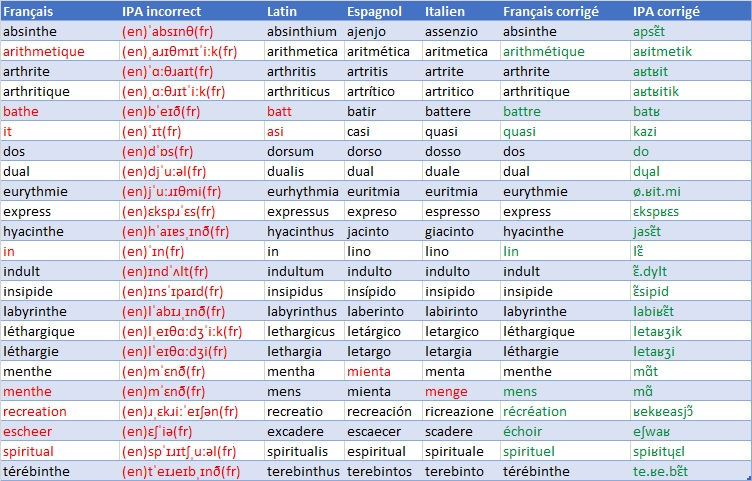
\includegraphics[width=0.8\textwidth]{figures/corrections_dataset.jpg}
    \caption{Tableau détaillant les corrections (en vert) apportées aux données du français. Les informations erronées sont en rouge.}
\end{figure}

\vspace{12pt}
Ensuite, un algorithme de détermination des candidats étant donné, un échantillon actuellement sélectionné et ses \glspl{cognat} associés a pu être établi. Une description est proposée dans l'annexe \ref{deter-candidats}\footnote{Elle aura eu l'intérêt d'apporter des détails qui ont été esquivés par \cite{he2022neural}.}.
Ce qu'il faut retenir est que le nombre de candidats à une certaine étape d'échantillonnage est dominé par un terme en $(2\sqrt{2})^d$, avec $d$ la plus grande \gls{edit_dist} entre la reconstruction actuelle et les \glspl{cognat}. Comme chaque candidat aura droit à sa probabilité calculée avec le programme dynamique fourni dans \autocite[section A.2]{he2022neural}, le temps d'exécution risque d'être coûteux. Le modèle a donc tout intérêt à ne pas débuter ses premiers échantillonnages à partir d'échantillons éloignés trop excessivement des \glspl{cognat}, d'où l'utilité des premières itérations d'un autre modèle de reconstruction pour l'initialisation.

\vspace{12pt}
Enfin, il a été possible de directement exploiter le code des chercheurs pour les programmes dynamiques, sur lesquels nous avions eu des difficultés de compréhension. Nous ne l'affichons donc pas dans le répertoire de Github, mais ce script a eu une importance centrale et a servi de base pour notre implémentation des inférences dans les modèles neuronaux d'édition.

\vspace{12pt}
Dans les fonctions qui restent à développer, une première doit effectuer le tirage aléatoire d'échantillons, qui sera simulé à l'aide d'une chaîne de Markov construite à partir de l'algorithme de Metropolis-Hastings \autocite{metro_has}, et dont la loi stationnaire finale sera donnée par l'équation ci-dessous, étant donné une variable aléatoire $X$ à laquelle on attribue le numéro de l'échantillon tiré dans la liste des $N$ candidats :
\begin{equation}
    p(X=i)=\frac{p(x_i|\{y_l, l\in L\})}{\sum_{j=1}^{N}p(x_j|\{y_l, l\in L\})}
\end{equation}
L'entraînement des modèles d'éditions à partir des données établies lors d'une espérance-maximisation est aussi encore à programmer. Pour terminer, l'entraînement des modèles de langue du latin n'a toujours pas été géré, de même que la construction des différents jeux de données pour le réaliser.

\chapter{Conclusion}
L'intelligence artificielle a déjà commencé sa révolution dans la linguistique historique. Les différents travaux étudiés ont montré que ces technologies ont su s'adapter aux contraintes du domaine en produisant des modélisations convenables, dans la limite où des données sur une langue sont disponibles. 

Bien que performants de par leur rapidité, il a été cependant démontré que les modèles neuronaux font des prédictions dont la fiabilité doit souvent être remise en question, du fait de la variété des cas possibles rencontrés dans une ou plusieurs langues, qu'ils savent difficilement gérer dans son ensemble. Néanmoins, des pistes de réflexion sont fournies aux linguistes grâce à ces outils, permettant de prétraiter leur travail.

L'amélioration du niveau de confiance qu'il sera possible d'accorder aux hypothèses sorties par les machines à base d'intelligence artificielle progressera certainement avec les avancées de la recherche sur la modélisation des langues en général, les progrès dans le domaine des langues contemporaines étant aussi importants à considérer que ceux dans le domaine des langues anciennes.

\printbibliography[heading=bibintoc]

\appendix

\chapter{Histoire de la linguistique historique} \label{histoire_LH}

\indent La linguistique historique aurait été introduite par Sir William Jones (1746-1794) lorsqu'il émet l'hypothèse que le grec, le latin et le sanskrit ont des origines communes, menant à une langue proto-indo-européenne. Une partie de ses hypothèses se seront révélées incorrectes plus tard, mais la langue proto-indo-européenne est toujours étudiée aujourd'hui, se voulant être la protolangue du latin, du gothique, du celte, du grec et du perse.  \\ \\ 
\indent Si toutes les langues indo-européennes descendent d'une langue primitive commune, quel était donc le peuple qui parlait cette langue, où se situait-il et à quelle époque ? Pour  essayer de répondre à cette question, on se base généralement sur des éléments de linguistique et d'archéologie. Plusieurs hypothèses existent, mais c'est actuellement l'hypothèse admise est que le proto-indo-européen viendrait d'un peuple semi-nomade ayant vécu il y a environ 6000 à 7000 ans dans la steppe située au nord de la Mer Noire, aux environs de  l'actuelle frontière entre la Russie et l'Ukraine. Ce peuple de guerriers et de cavaliers conquérants aurait entrepris de nombreuses migrations, permettant ainsi la diffusion de leur langue en Europe et en Asie.

\chapter{Phonologie et Phonétique} \label{phonologie_phonetique}

\indent Pour la description de l'appareil, nous nous référerons une figure schématique, où $A$ désigne la cavité nasale, $B$ la cavité buccale, $C$ le larynx, contenant la glotte $\varepsilon$ entre les deux cordes vocales.\\
\indent Dans la bouche on distingue les lèvres $\alpha$ et $a$, la langue $\beta$ - $\gamma$ ($\beta$ désignant la pointe et $\gamma$ tout le reste), les dents supérieures $d$, le palais, comprenant une partie antérieure, osseuse et inerte $f$ et $h$, et une partie postérieure, molle et mobile ou voile du palais $i$, enfin la luette $\delta$. \\ 
\indent Les lettres grecques désignent les organes actifs dans l'articulation, les lettres latines les parties passives. La glotte $\varepsilon$, formée de deux muscles parallèles ou cordes vocales, s'ouvre par leur écartement ou se ferme par leur resserrement. La fermeture complète n'entre pour ainsi dire pas en ligne de compte ; quant à l'ouverture, elle est tantôt large, tantôt étroite. Dans le premier cas, l'air passant librement, les cordes vocales ne vibrent pas ; dans le second, le passage de l'air détermine des vibrations sonores. Il n'y a pas d'autre alternative dans l'émission normale des sons. La cavité nasale est un organe tout à fait immobile ; le passage de l'air peut être arrêté par le relèvement de la luette $\delta$, rien de plus ; c'est une porte ouverte ou fermée.\\

\indent Le système phonologique français est composé de 35 phonèmes : $17$ sont dits consonantiques ; ils mettent en jeu les $20$ consonnes de l'alphabet, $15$ sont dits vocaliques ; ils mettent en jeu les $6$ voyelles de l'alphabet et $3$ semi-consonantiques ou semi-vocaliques.\\

\indent \textbf{Phonème consonantique} : [ p ] de paon, [ f ] de faon,  [ b ] de banc, [ v ] de vent, [ t ] de temps [ d ] de dent, [ s ] de sans, [ z ] de zan, [ \textesh  ] de chant [ \textyogh  ] de Jean,  [ g ] de gant, [ k ] de quand,  [ l ] de lent, [ \textscr ] de rend,  [ m ] de ment, [ n ] de non,  [ \textltailn ] de pagne \\ 
\indent \textbf{Phonèmes vocaliques} :  [ a ] de patte, [ \oe ] de \oe uf, [ \o ] de feu, [ \~a ] de pente [ o ] de côte, [ \textschwa  ] de petit, [ o ] de cotte, [ e ] de pré, [ \~{\textopeno} ] de conte, [ $\varepsilon$ ]  de prêt [ i ] de nid, [ $\varepsilon$ ]   de brin, [ y ] de nu, [ \~{\oe} ] de brun, [ u ] de nous. \\ 
\indent \textbf{Phonème semi-consonantique ou semi-vocalique} : [w] de oui, [j] maille, [\textturnh] de pluie.\\

\chapter{Quelques principes de changements de phonèmes} \label{changement_phonetique}

\textbf{La palatalisation} : La palatalisation est un processus phonétique qui consiste à prononcer une consonne avec un son de palais mou. Par exemple, en ancien français, le son "ch" était prononcé "k" dans certains mots, mais a évolué vers un son de palais mou en français moderne, comme dans le mot "chien".\\

\textbf{La diphtongaison} : La diphtongaison est un processus phonétique qui consiste à ajouter un deuxième son vocalique à la fin d'un son vocalique existant. Par exemple, en ancien français, le son "i" dans le mot "pierre" était prononcé comme une voyelle simple, mais a évolué vers un son diphtongué "ie" en français moderne.\\

\textbf{La disparition de voyelles} : La disparition de voyelles est un processus phonétique qui consiste à éliminer une voyelle en position finale ou médiane d'un mot. Par exemple, le mot "femme" était autrefois prononcé avec une voyelle en position médiane, mais cette voyelle est tombée au fil du temps, laissant le mot avec deux consonnes.\\

\textbf{La liaison} : La liaison est un processus phonétique qui consiste à lier la dernière consonne d'un mot avec la première voyelle du mot suivant. Par exemple, dans la phrase "les amis", la liaison est faite entre le "s" de "les" et le "a" de "amis".\\ 

\textbf{La nasalisation} : La nasalisation est un processus phonétique qui consiste à produire un son nasal en passant de l'air par les fosses nasales. Par exemple, en français, les voyelles suivant une consonne nasale, comme le "n" ou le "m", sont nasalisées, comme dans le mot "enfant".

\chapter{Fine-tuning} \label{fine-tuning}

\indent Actuellement, en traduction automatique, le modèle neuronal de type encodeur-décodeur le plus utilisé sont les Transformeurs \ref{transformers} qui ont su montré leur performance dans la tâche de traduction automatique. L'une des raisons de ces résultats est qu'ils peuvent être entraînés sur de grande quantité de données, et se crée une \og bonne\fg{} représentation de celles-ci.\\
\indent Mais, dans le cadre de la reconstruction d'une langue, il faut s'attendre à avoir \textit{peu} (ou pas) de données sur la langue à reconstituer. Dans notre cas, nous souhaitons reconstruire le latin à partir de langue romanes (français, espagnol, italien, portugais), dont nous possédons une base de données contenant environ 5 000 mots phonétisés par langue (latin inclus). Cette base de données est très petite face aux quantités gigantesques (environ des millions de mots) que peuvent traiter les grands modèles de langue.\\
\indent Ainsi, nous avons décidé d'utiliser des modèles multilingues pré-entraînés dans la tâche de traduction. En effet, pour pallier le \og manque\fg{} de données d'entraînement, et espérer utiliser les représentations que ce sont construits ces modèles, c'est-à-dire, les relations sémantiques et syntaxiques qu'ils ont pu apprendre, il a été choisi d'utiliser des modèles qui ont déjà été entraînés sur de grandes quantités de données dans les langues romanes. Ici, nous avons choisi les modèles \textit{mBart} \autocite{mbart} et \textit{mT5} \autocite{mt5} de la librairie \textit{transformers} de \textit{HuggingFace} \autocite{hf_lib_transformer}, qui respectent les critères précédents\footnote{Les modèles choisis ne sont pas directement ces modèles, mais des modèles reprenant la même architecture affinés pour la tâche de traduction.}.\\ 
\indent Maintenant, nous devons affiner \textit{fine-tuning} les modèles choisis pour notre tâche de reconstruction, c'est-à-dire, que nous allons continuer l'entraînement de ces modèles pré-entraînés avec notre base de données pour qu'ils effectuent la tâche de reconstruction. L'affinement d'un modèle neuronal est un procédé courant quand on souhaite utilisé l'apprentissage (les connaissances) d'un modèle pour l'adapter à la tâche souhaitée (similaire à la tâche initial), surtout quand on ne possède pas assez de données pour entraîner notre modèle en partant de zéro. À préciser que ces modèles ont été pré-entraînés sur des données orthographiques, et non phonétiques, ainsi, pour espérer utiliser les représentations de ces modèles, nous avons fournis notre base de données orthographiques.\\
\indent La mise en place de l'approche s'est effectué par le téléchargement des modèles, puis la configuration de leur entraînement supervisé et de leur évaluation (par \gls{edit_dist} \autocite{levenshtein}).\\
\indent Après plusieurs tests d'affinement et d'optimisation d'hyperparamètres de nos modèles, nous n'avons obtenus aucun résultat concluant\footnote{Une des causes supposées était que les modèles étaient trop grands pour apprendre avec notre base de données, ainsi, des versions plus petites ont été utilisé \textit{tiny-mbart} (\url{https://huggingface.co/sshleifer/tiny-mbart}) et \textit{mT5-small} (\url{https://huggingface.co/google/mt5-small}), sans pour autant obtenir de résultats significatifs.}. Plusieurs causes sont possibles, d'abord le manque de données d'entraînement empêchant le modèle d'apprendre la tâche demandée\footnote{Possible que les modèles apprennent avec de plus grandes quantités de données, mais nous sortons du cadre de notre étude consistant à travailler avec des langues où l'on possède peu de données.}, on sait d'ailleurs que les Transformeurs (et cela est amplifié quand on utilise des grands modèles de langue) ne sont pas très bon dans des situations à basses ressources, mais aussi la supposition que la tâche de traduction automatique est proche de la tâche de reconstruction, enfin on ne repose plus sur le principe de régularité de changement phonétique en travaillant qu'avec des données orthographiques (dont les changements sont plus irréguliers) ainsi il est plus difficile pour nos modèles d'apprendre la tâche. Par conséquent, nous en concluons que l'utilisation de Transformeurs n'est pas approprié pour notre tâche de reconstruction, nous devons nous tourné vers d'autres type de modèle.

\chapter{Détermination des n\oe{}uds dans des chemins d'édition de taille minimale.} \label{deter-candidats}

Soient $x$ et $y$ deux chaînes de caractères quelconques. L'objectif est de trouver toutes les chaînes intermédiaires qui ont possiblement été créées pour transformer $x$ en $y$ avec le nombre minimal de modifications appliquées à $x$. Dans l'illustration de \cite{he2022neural} ci-dessous, les éléments à trouver sont ceux entre \og{} abs\textepsilon{}ns \fg{} et \og{} ass\textepsilon{}nte \fg{}\footnote{Les mots \og{} abs\textepsilon{}nts\fg{} et \og{} ass\textepsilon{}nts\fg{} devraient y être ajoutés pour obtenir l'ensemble des solutions.}. 

\begin{figure}[!h]
    \centering
    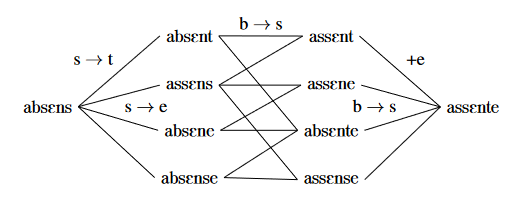
\includegraphics[width=0.7\textwidth]{figures/fiure_5_he.png}
    \caption{Représentation des intermédiaires possibles (figuré de \cite{he2022neural}). Ils sont obtenus par application de modifications faisant partie d'un chemin d'édition de taille minimale (ici de 3)}
    \label{fig:illustratin_he}
\end{figure}

La taille minimale des chemins d'édition est donnée par la \gls{edit_dist} entre les deux chaînes, en choisissant d'attribuer à la substitution un coût d'opération de 1, égal à celui de l'insertion et de la suppression. Le calcul de cette valeur $d$ s'effectue avec un programme dynamique proposé par \cite{levenshtein}. On pose $M$ sa matrice de calcul associée, de dimension $(|x|+1, |y|+1)$\footnote{avec $|a|$ qui désigne ici le nombre de caractères de la chaîne $a$} et dont le coefficient $M[i,j]$ à la ligne $i$ et à la colonne $j$ contient la distance d'édition entre les $i$ premiers caractères de x ($x[:i]$) et les $j$ premiers caractères de $y$ ($y[:j]$) (pour $i \in [\![0,|x|]\!]$ et $j \in [\![0,|y|]\!]$). 

On parcourt récursivement $M$ à partir de la position $(|x|, |y|)$ de sorte à établir toutes les combinaisons possibles de $d$ modifications à appliquer à $x$ pour obtenir $y$. Il sera alors possible de modéliser chaque modification distincte afin de pouvoir appliquer chacune d'elle indépendamment sur $x$. À chaque combinaison de $k$ modifications appliquées à $x$, avec $k$ entre 1 et $d-1$ compris, un nouvel intermédiaire est calculé. Toutes les combinaisons seront donc déterminées.

\section{Parcours matriciel}

Les insertions, substitutions et suppressions de caractères à effectuer pour modifier le moins possible $x$ s'identifient en remontant la matrice $M$. Si on note $n$ le coefficient de $M$ qui est rencontré à un certain moment dans le parcours, il est possible de s'assurer que le chemin emprunté balaiera toujours une séquence de $d$ éditions ayant transformé $x$ vers $y$ dès lors qu'on s'oriente toujours vers \og{} le haut et la gauche \fg{} et que $n$ diminue en permanence. \autocite[chap. 2]{jurafsky} On créé un graphe orienté $G$ ne contenant d'abord qu'un n\oe{}ud vide $O$ et dans lequel on stocke les modifications trouvées. Pour $n=M[i,j]$, l'algorithme de parcours est alors le suivant :
\begin{itemize}
    \item si $n=0$, l'algorithme est terminé.
    \item sinon, \begin{itemize}
        \item si $M[i-1, j-1] = n-1$, alors le caractère $x[i]$ a été substitué par le caractère $y[j]$. On ajoute cette modification en tant que n\oe{}ud du graphe, en le connectant au noeud actuel et on poursuit récursivement le parcours à la position $(i-1, j-1)$.
        \item si $M[i-1, j] = n-1$, alors l'insertion au moins du caractère $y[j]$ a eu lieu après le caractère $x[i]$. Les mêmes actions que précédemment sont effectuées, sauf qu'on poursuit le parcours à la position $(i-1, j)$
        \item si $M[i, j-1] = n-1$, alors le caractère x[i] a été supprimé. On ajoute cette modification au graphe de la même façon et on poursuit le parcours à la position $(i, j-1)$
    \end{itemize}
\end{itemize}
Pour les deux chaînes du figuré \ref{fig:illustratin_he}, le parcours effectué dans la matrice et le graphe d'édition construit sont illustrés dans le figuré ci-dessous.
\begin{figure}[!h]
    \centering
    \begin{subfigure}[b]{0.4\textwidth}
        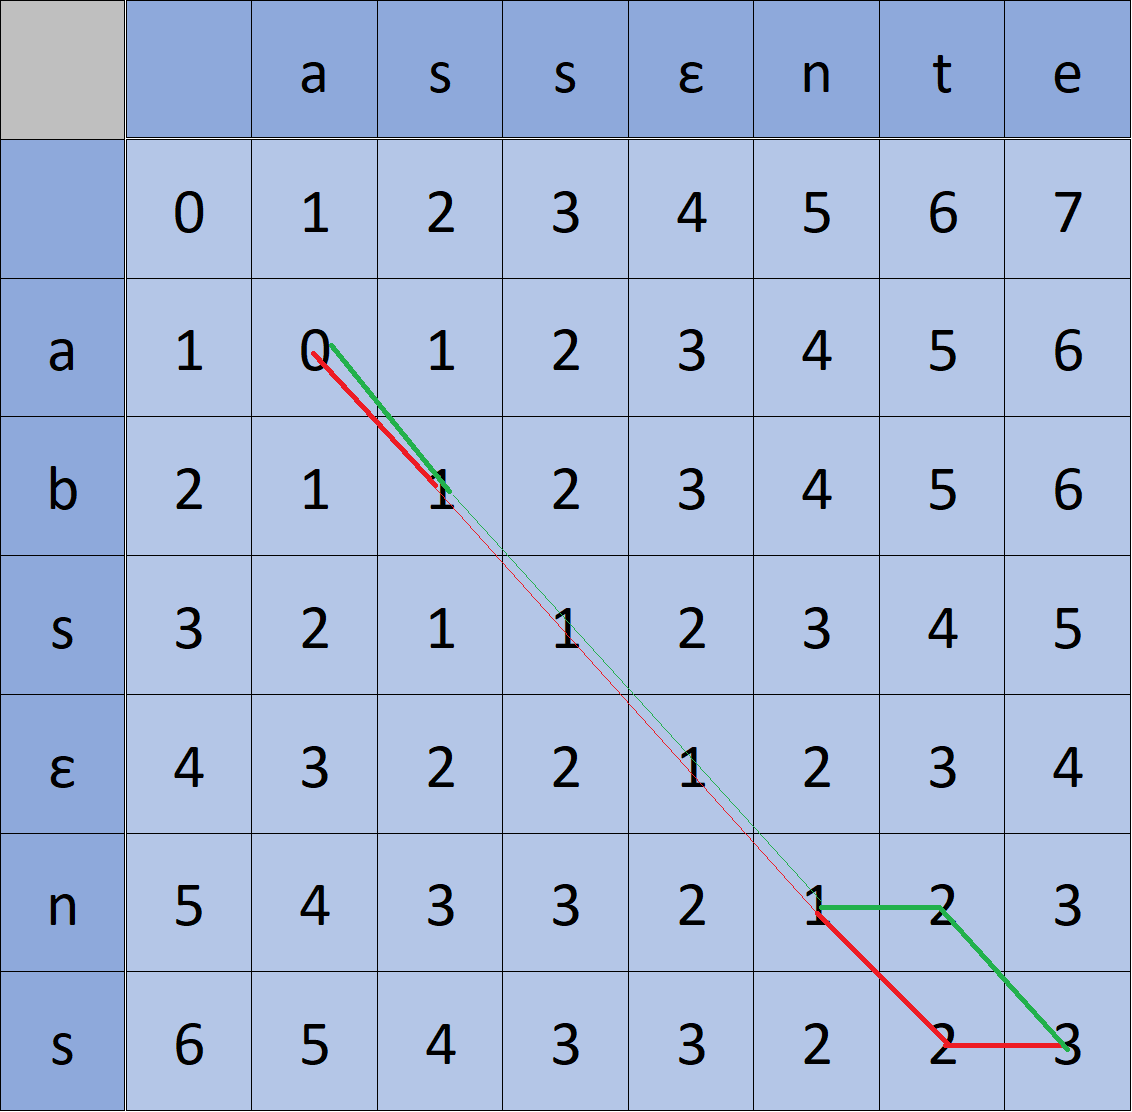
\includegraphics[width=\textwidth]{figures/tab_editions.png}
        \caption{Illustration du parcours de la matrice de calcul de la distance d'édition pour les mots \og{} abs\textepsilon{}nts\fg{} et \og{} ass\textepsilon{}nts\fg{}}
    \end{subfigure}
    \begin{subfigure}[b]{0.4\textwidth}
        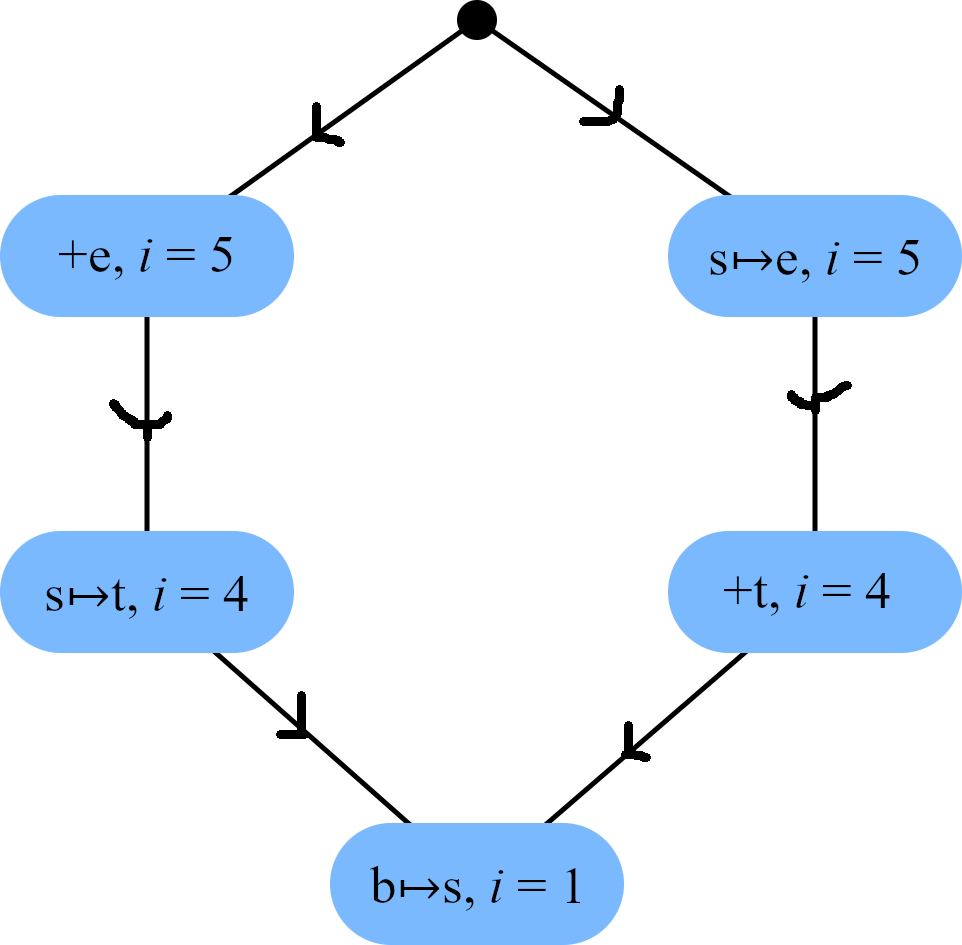
\includegraphics[width=\textwidth]{figures/graphe modifs assente.png}
        \caption{Représentation du graphe d'édition calculé pour les mots \og{} abs\textepsilon{}nts\fg{} et \og{} ass\textepsilon{}nts\fg{}}
    \end{subfigure}
    
\end{figure}

\section{Modélisation d'une modification}

Avec la représentation par un graphe des modifications comme illustrée ci-dessus, presque toutes les informations sont correctement définies pour construire les intermédiaires. Cependant, dans le cas où plusieurs caractères ont été insérés à la même position $i$ de $x$, il faut veiller à ce qu'ils restent ordonnés correctement dans l'intermédiaire produit, indépendamment de l'ordre avec lequel les insertions seront appliquées à $x$ --- puisqu'il est intéressant ici de travailler avec des combinaisons de modifications. Il est donc nécessaire d'ajouter une propriété supplémentaire lors de l'étiquettage des n\oe{}uds. La position $j$ dans $y$ du caractère inséré répond à cette demande, d'autant plus que disposer de la coordonnée du coefficient de la matrice $M$ à partir duquel une modification a été identifiée permet de distinguer des modifications impliquant des caractères identiques dans des chemins d'édition différents, évitant alors à ces chemins d'être croisés à tort (ce cas a déjà été rencontré lors du développement de l'algorithme).

\section{Combinaisons d'éditions}

À partir du graphe orienté, il est possible grâce à un parcours en largeur depuis le n\oe{}ud vide $O$ d'établir toutes les combinaisons de $k$ modifications distinctes parmi les ensembles à $d$ éléments qui correspondent avec les chemins d'édition, après quoi toutes les chaînes intermédiaires sont déterminables.\\
L'algorithme permet d'établir toutes les combinaisons sans doublon. Pour chaque n\oe{}ud $N$, d'une profondeur $k$\footnote{i.e. qu'il est possible de le rejoindre depuis $O$ en traversant $k$ arêtes orientées} et dont on note $u$ la modification contenue dans l'étiquette, les seules combinaisons construites sont en effet les unions du singleton $\{u\}$ avec les combinaisons construites auparavant par l'ensemble des sommets ancestraux à $N$ (i.e. ceux d'une profondeur entre 0 et $k-1$ inclus, qui auront été obligatoirement déjà traités puisque le parcours du graphe s'effectue en largeur). Puisque $u$ n'a pas été vu par ces sommets-ci, les nouvelles combinaisons sont donc bien distinctes de celles construites précédemment, de mêmes que celles construites chez les autres sommets avec la même profondeur $k$.\\
Néanmoins, plusieurs combinaisons distinctes de modifications peuvent déboucher sur le même intermédiaire généré. Des améliorations dans l'étape de l'établissement des combinaisons est donc à faire afin de s'assurer de ne sortir que des intermédiaires uniques.\\

Dans le meilleure des cas, le graphe d'édition forme un simple chemin. Le nombre de combinaisons construites sera alors de
\begin{equation}
    \sum_{k=0}^{d} {{d}\choose{k}} = 2^d
\end{equation}
En revanche, en pratique, il est fréquent que des chemins se séparent en deux, ce qui implique que le nombre de candidats peut être plus important. Cette séparation est cependant nécessairement suivie d'un renouement plus en profondeur dans le graphe, puisque les chemins d'édition mènent tous à l'obtention de $y$ (voir le figuré \ref{fig:complex_graph} pour un exemple). De plus, l'observation de graphes d'édition pour d'autres mots semble confirmer qu'un n\oe{}ud ne puisse pas réunir plus de deux chemins.\\
Étant donné ces conditions, le graphe imaginable avec un nombre maximal de sommets pour une distance d'édition $d$ fixée est celui dont le nombre de sommets est multiplié par deux à chaque descente en profondeur sur la première moitié du graphe pour ensuite être divisé par deux sur l'autre moitié, où les chemins fractionnés se réunissent à nouveau. Dans cet exemple de graphe, il va être montré que le nombre de combinaisons calculées est dominé par une valeur allant au-delà de $O(2^d)$. Déterminer si cette valeur constitue une majoration de la quantité d'intermédiaires générés est un problème mathématique dont le traitement est ici laissé pour des recherches ultérieures.

Soit $(c_k)_{0 \leq k \leq d}$ la suite des nombres de combinaisons générées par l'algorithme lorsqu'il travaille sur un n\oe{}ud de profondeur $k$ et soit $(n_k)_{0\leq k \leq d}$ celle des nombres de sommets que le graphe possède à cette même profondeur. On a donc $c_0 = n_0 = 1$. À une profondeur $k \in [\![1,\lceil \frac{d}{2}\rceil]\!]$, un sommet est situé sur un chemin simple et le nombre de combinaisons qui y sont générées est alors de $c_k = 2^{k-1}$. Puisque le nombre de sommets est multiplié par deux d'une profondeur $k$ à $k+1$, pour $k \leq \lceil \frac{d}{2}\rceil -1$, on a donc $n_k=2^k, \forall k\leq \lceil \frac{d}{2} \rceil$.\\
Pour $k > \lceil \frac{d}{2} \rceil $, si on note $m:=k-\lceil \frac{d}{2} \rceil$, on démontre sans mal que $n_{(\lceil \frac{d}{2} \rceil + m)} = 2^{\lceil \frac{d}{2}\rceil - m}$. Chaque n\oe{}ud renoue deux sommets de sorte à avoir le plus de sommets ancestraux possibles, dont le nombre à la profondeur $j$ est alors de $\min\{2^{m}, n_j=2^{j}\}$, dans le cas où $j\leq \lceil \frac{d}{2} \rceil$ sinon de $2^{k-j}$, pour $\lceil \frac{d}{2} \rceil < j <k$.
Le nombre de combinaisons dans un n\oe{}ud à la profondeur $k$ vaut donc, $\forall 1 \leq m \leq \lceil \frac{d}{2} \rceil$ :
\begin{equation} \label{eq:def_combis_2}
    \begin{split}
        c_k = c_{(\lceil \frac{d}{2} \rceil + m)} = & \sum_{j=0}^{m-1} 2^j c_j + \sum_{j=m}^{\lceil \frac{d}{2} \rceil} 2^m c_j + \sum_{j=\lceil \frac{d}{2} \rceil+1}^{k-1}2^{k-j}c_j \\
        = & 1 + \sum_{j=1}^{m-1} 2^j 2^{j-1} + 2^m\sum_{j=m}^{\lceil \frac{d}{2} \rceil} 2^{j-1} + \sum_{p=1}^{m-1} 2^{m-p}c_{(\lceil \frac{d}{2} \rceil + p)}\\
        = & 1 + \frac{1}{2}\sum_{j=1}^{m-1} 4^{j} + 2^m\left(2^{\lceil \frac{d}{2} \rceil} -2^{m-1} + \sum_{p=1}^{m-1} 2^{-p}c_{(\lceil \frac{d}{2} \rceil + p)}\right)\\
    \end{split}
\end{equation}
Pour $m=1$, on a alors $c_{(\lceil \frac{d}{2} \rceil + 1)} = 1 +2\left(2^{\lceil \frac{d}{2} \rceil} - 1\right) = 2^{\lceil \frac{d}{2} \rceil+1}-1$ et on a donc bien ${c_{(\lceil \frac{d}{2} \rceil + 1)} = 2(2c_{(\lceil \frac{d}{2} \rceil)})-1}$, ce qui confirme que les combinaisons calculées dans les premiers sommets de renouement sont bien générés à partir de l'union de deux ensembles de combinaisons calculées sur des chemins d'édition simples de longueur allant jusqu'à $\lceil \frac{d}{2} \rceil$, dont le cardinal de chacun vaut $2c_{(\lceil \frac{d}{2} \rceil)} = 2^{\lceil \frac{d}{2} \rceil}$. Ces deux ensembles contiennent seulement la combinaison vide en commun. Le cardinal de l'union vaut donc le double des cardinaux auquel on ôte 1.\\
Pour $m > 1$, la réécriture suivante est valide :
\begin{equation} \label{eq:combis_m2}
    \begin{split}
        c_k = c_{(\lceil \frac{d}{2} \rceil + m)} = & 1 + \frac{1}{2}\left(\frac{4^m - 1}{3}-1\right) -\frac{1}{2}4^m + 2^m\left(2^{\lceil \frac{d}{2} \rceil} + \sum_{p=1}^{m-1} 2^{-p}c_{(\lceil \frac{d}{2} \rceil + p)}\right)\\
        = & \frac{1}{3}(1-4^m) + 2^m\left(2^{\lceil \frac{d}{2} \rceil} + \sum_{p=1}^{m-1} 2^{-p}c_{(\lceil \frac{d}{2} \rceil + p)}\right)
    \end{split}
\end{equation}
En notant $(v_m)_{1 \leq m \leq \lceil \frac{d}{2} \rceil}$ la suite $(c_{(\lceil \frac{d}{2} \rceil+m)})_{1 \leq m \leq \lceil \frac{d}{2} \rceil}$, il est ainsi possible de déterminer une relation de récurrence entre les termes, pour $m \geq 2$ :
\begin{equation} %TODO corriger la constante
    \begin{split}
        v_{m+1} = & \frac{1}{3}(1-4^{m+1}) + 2^{m+1}\left(2^{\lceil \frac{d}{2} \rceil} + \sum_{p=1}^{m} 2^{-p}v_p\right) = \frac{1 - 4\cdot4^m}{3} + 2\cdot{}2^{m}\left(2^{\lceil \frac{d}{2} \rceil} + \sum_{p=1}^{m-1} 2^{-p}v_p + 2^{-m}v_m\right) \\
        = & \frac{1 - 4\cdot4^m}{3} + 2\cdot{}2^{m}\left(2^{\lceil \frac{d}{2} \rceil} + \sum_{p=1}^{m-1} 2^{-p}v_p\right) + 2v_m = \frac{1 - 4\cdot4^m}{3} + 2\left(v_m - \frac{1-4^m}{3}\right) + 2v_m \\
        = & 4v_m - \frac{2}{3}4^m - \frac{1}{3}
    \end{split}
\end{equation}
On déduit donc une expression explicite pour $(v_m)_{2\leq m \leq \lceil \frac{d}{2} \rceil}$\footnote{On s'intéresse évidemment à étudier des valeurs infinies de $d$, ce qui ne pose donc pas de problème pour définir $(v_m)_{2\leq m \leq \lceil \frac{d}{2} \rceil}$}:
\begin{equation}
    v_m = 4^{m-2} v_2 + \sum_{j=2}^{m-1}\left(\frac{-2}{3}4^j - \frac{1}{3}\right)4^{m-1-j}
    = 4^{m-2} v_2 - \frac{2}{3}(m-2)4^{m-1} - \frac{1}{3}4^{m-3}\sum_{j=0}^{m-3}4^{-j}
\end{equation}
D'après l'équation \ref{eq:combis_m2} et l'expression de $c_{(\lceil \frac{d}{2} \rceil +1)}$, on a $v_2 = 2^{\left(\lceil \frac{d}{2}\rceil + 3\right)}-7$. Pour $m\geq 3$, on obtient donc :
\begin{equation}
    \begin{split}
        v_m = & 4^{m-2}\left(2^{\left(\lceil \frac{d}{2}\rceil + 3\right)}-7\right) - \frac{2}{3}(m-2)4^{m-1} - \frac{1}{3}4^{m-3}\frac{4}{3}(1-4^{2-m})\\
        \textrm{D'où, } v_m = c_{\left(\lceil\frac{d}{2}\rceil + m\right)} = & 2^{\left(2m + \lceil \frac{d}{2}\rceil - 1\right)} - \frac{2}{3}m4^{m-1} - \frac{4^m -1}{9}
    \end{split}
\end{equation}

La quantité totale de combinaisons construites avec le graphe est donnée par la somme ${N=\sum_{k=0}^{d}n_kc_k}$.
Si $d$ est paire, on remarque alors à partir de la première expression dd l'équation \ref{eq:def_combis_2} que ${N=2*c_d}$. Si $d$ est impaire, on remarque de la même façon que ${N=c_{d+1}}$ Dans tous les cas, on a donc
\begin{equation}
    N=O(c_{2\lceil\frac{d}{2}\rceil})=O(v_{\lceil\frac{d}{2}\rceil}), \textrm{avec }v_{\lceil\frac{d}{2}\rceil} = \frac{1}{2}2^{3\lceil\frac{d}{2}\rceil} - \frac{1}{12}2\lceil\frac{d}{2}\rceil2^{2\lceil\frac{d}{2}\rceil} -\frac{1}{9}2^{2\lceil\frac{d}{2}\rceil} + \frac{1}{9} = O(2^{\frac{3}{2}d})
\end{equation}


\begin{figure}[h]{} 
    \centering
    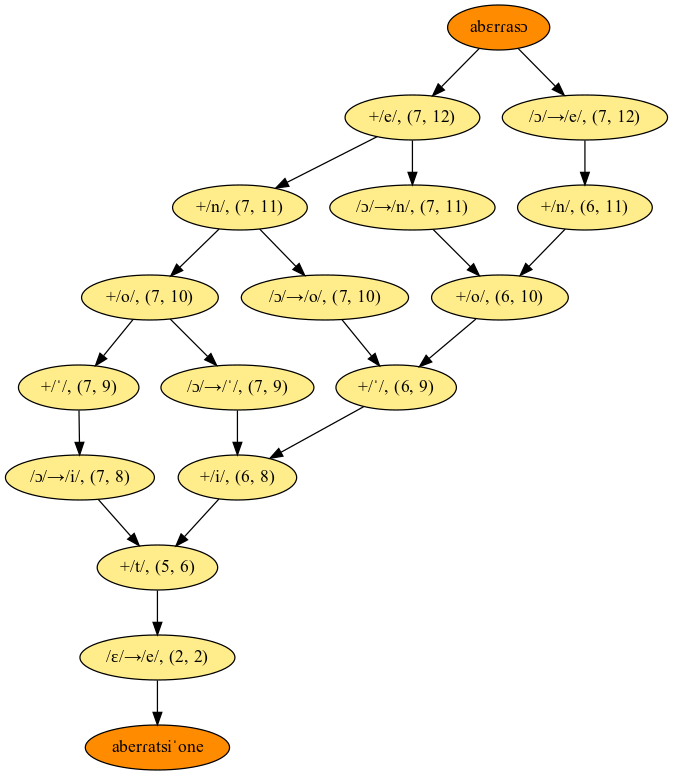
\includegraphics[width=0.7\textwidth]{figures/graphe_complexe.png}
    \caption{Représentation d'un graphe d'édition plus complexe.}
\end{figure} \label{fig:complex_graph}

\end{document}